%%%%%%%%%%%%%%%%%%%%%%%%%%%%%%%%

% The golden age of sequence analysis

%%%%%%%%%%%%%%%%%%%%%%%%%%%%%%%%

\chapter[The golden age of sequence analysis]{\textbf{T}he golden age\\of sequence analysis}\label{sec:algorithms}
\sectionorange*{Summary}
\begin{center}
\begin{tabular}{c}
\fcolorbox{blue}{verylightgrey}{
\begin{minipage}[][4cm][c]{0.8\linewidth}
\sffamily
%abstract 
This chapter aims to be a historical survey of the sequence comparisons algorithms analyzing the most 
relevant solutions. The algorithms that represented innovative changes in the field are described in detail,
covering the concepts of global, local and multiple alignment of sequences. In addition, the theoretical 
framework of the map alignment problems necessary to understand the rest of work presented in this thesis 
is also formalized here.
\end{minipage}}\\
\\[2ex]
\begin{minipage}[][4cm][c]{1.1\linewidth}
\minitoc
\end{minipage}
\end{tabular}
\end{center}
\newpage



\sectionorange{Foundations of sequence comparison}\label{sec:history}

\lettrine[lines=4,loversize=-0.1,lraise=0.1,lhang=.2]{T}{he topic of biosequence comparison} has a rich 
history dating back over 40 years. It is certainly very difficult to trace a line in some moments to 
establish the order in which every new development was presented because of the enormous body of
publications that have contributed substantially to improve this field. Several general reviews have been 
used to reconstruct the history of biological sequence comparisons 
\citet{mount:2001a,myers:1991a,ouzounis:2003,sankoff:1983a,meidanis:1997a, waterman:1984a}. 

Molecular evolution began to be studied in the 1960s when a few protein sequences were available, being
published into the protein sequence atlas \citep{dayhoff:1965a}. Soon, pioneering analysis appeared to 
infer the evolutionary relationships from these sequences, depicted as distances in phylogenetic trees 
\citep{fitch:1967a}. 

Outside the molecular biology, other significant advances in mathematics and in the emerging discipline of
computer science contributed decisively to the current state of the art. For instance, it is impossible to 
understand the history of modern sequence alignment without mentioning the birth of a new technique in the
1950s to solve multistage decision process problems called dynamic programming \citep{bellman:1957a,dreyfus:2002a}. 
A problem is solved by dynamic programming if the answer can be efficiently determined by computing a table of 
optimal answers to progressively larger subproblems. The principle of optimality requires that the optimal answer 
to a given subproblem is expressible in terms of optimal answers to smaller subproblems. During all this time, 
despite innumerable optimal and heuristic approaches have been proposed to obtain the best alignments between 
two sequences with the minimum cost, dynamic programming is still the most stable technique to solve the original 
problem and many of its variations.

Another key concept is the definition of several metrics of distance between sequences in the coding 
theory field. Since noise in a transmission channel introduces errors into the signal reception, several
mechanisms were developed for detection and correction of such errors. The Hamming distance, defined as the 
number of positions in which two sequences differ, was oriented to detect only substitutions \citep{hamming:1950a}. 
Next, \citet{levhenshtein:1966a} presented the edit distance, which was the earliest known use of a distance 
function that is appropriate to detect insertions and deletions of symbols in the original message.
 
It is not clear when the basic dynamic programming algorithm for molecular sequence comparison first 
appeared. It was probably rediscovered many times in different contexts. The well-known paper by
\citet{needleman:1970a} who presented an algorithm for maximizing the number of matches minus the number
of insertions and deletions is generally considered to be the first important contribution. Although no 
complexity analysis was provided, the original \citeauthor{needleman:1970a} algorithm measured the
homology between two sequences in a $O(n^3)$ time.

A more rigorous approach with solid mathematical foundations arised from the problem of computing the 
distance between two sequences \citep{ulam:1972a,beyer:1985a}. \citet{sellers:1974a} presented a dynamic
algorithm based on the Levhenshtein metric distance. Though less flexible for future variations of the 
problem, this new approach fitted better with the perspective of evolutionary distance analysis 
developed earlier. Under the realistic assumption that both sequences have $n$ nucleotides, the 
\citeauthor{sellers:1974a} algorithm have computation time proportional to $O(n^2)$. A comprehensive 
study of equivalence between similarity and distance was presented in \citet{smith:1981b}. 

Within the field of computer science, sequence comparison appeared in simpler incarnations of the 
molecular biology problems, for comparing the contents of files or correcting the spelling of words. For example, 
the longest common subsequence problem (LCS) consists on finding an alignment that maximizes the number of
identical aligned pairs between two sequences (see \citet{apostolico:1987a} for a review).
Interestingly for long sequences, \citet{hirschberg:1975a} applied the divide and conquer strategy to 
solve the LCS problem in $O(2 n^2)$ time with a linear space cost instead of the established quadratic cost.
\citet{myers:1988a} generalized this technique to align two sequences using $O(n)$ space.

Nonetheless, the treatment of gaps was still biologically unrealistic as a deletion of $n$ symbols and $n$ 
deletions of one symbol were punished indistinctly. \citet{waterman:1976a} accommodated the same 
algorithm to deal with multiple deletions and insertions, introducing the concept of general gap 
penalty functions. \citet{gotoh:1982a} reduced the asymptotic cost from $O(n^3)$ to $O(n^2)$, under the
application of the affine gap penalty functions in which there was an initial penalty for opening a gap 
and an additional minor penalty for extending an existent one. Apart from general and affine gap functions, 
\citet{waterman:1984a} introduced the concept of concave gap function in which the cost of extending an 
existent gap grows with the logarithm of the length of the gap as a continuous curve. Later, \citet{eppstein:1988a} 
and \citet{miller:1988a} independently arrived at $O(n^2 \log{n})$ solutions of the problem.

DNA and protein sequences are the result of an evolutionary process that tend to preserve those
parts that are key to perform a function, permitting variation in the rest. Thus a global comparison
can easily produce a very poor alignment of two sequences that have some parts in common while others
are completely free of conservation. \citet{smith:1981c} introduced the concept of local alignment
with a simple variation in the basic global similarity algorithm without increasing its cost. Under the 
premise of a negative gap penalty, reported alignments are regions of high similarity with a positive 
score within. \citet{sellers:1984a} tried to export the same concept to the distance metric. Only, those 
paths in the matrix whose density of mismatches was below a certain threshold were reported.

Thousands of genomic and proteomic sequences, that is millions of nucleotides and amino acids,
are rapidly being accumulated in the biological databases. However, searching a database with a query 
sequence for similarities to other sequences using the optimal algorithms enumerated above
is clearly unfeasible when this simple operation involves thousands of comparisons between two sequences.
To overcome this problem, a new family of heuristic procedures that produce nearly correct answers in
a simple and cheaper fashion was designed. The most popular representatives of these are the program
FASTA \citep{pearson:1988a} and the program BLAST \citep{altschul:1990a}. The FASTA heuristic is based
on identifying the identities between two sequences (diagonals in the matrix) and then applying 
some more expensive procedures only on those subalignments. BLAST processing relies on first, detecting
ungapped segment pairs of high score and then, extending them from both ends until a threshold value
is reached. 

A collateral effect of producing hundreds of alignments was the concern about the quality of a
given alignment between two sequences. The significance of a local alignment score can be tested by 
comparing with the distribution of scores expected by aligning two random sequences with the same length 
and composition \citep{karlin:1990a}. These random sequence alignment scores follow a distribution called
the extreme value distribution (also known as the Gumbel distribution), which is similar to a normal
distribution but with a positively skewed tail in the higher score \citep{gumbel:1962a}. Less interest 
has traditionally been focused on global comparisons because of a global alignment is always produced by 
definition even between random or unrelated sequences, growing the score proportionally to the length of 
them.

In attempt to distinguish more distant relationships, the implementation of comparisons for more than 
two sequences is the logical evolution to locate elements with function that are conserved for instance 
in several homologous sequences.
\citet{waterman:1976a} naturally extended the basic dynamic programming recurrence for $k$ sequences, with
an exponential cost $O(n^k)$. As this approach is generally impractical, some heuristics
appeared to solve the problem with a minor cost. The most popular of them is the hierarchical or 
clustering method called progressive alignment that first takes $O(k^2 n^2)$ to perform all pairwise 
alignments and second, produce a multiple alignment following a guide tree to merge these alignments 
\citep{feng:1987a}. The program CLUSTALW \citep{thompson:1994a} combines this strategy with different 
weighting schemes according to the progression in the distances tree. Previously, \citet{carrillo:1988a} 
developed another method based on identifying the projections of the pairwise alignments that can form the multiple 
alignment. Moreover, hidden Markov models have been used to produce multiple alignments of a family of
sequences to which more members can be dynamically be added (profile HMMs, see \citealp{durbin:1998a}).

Pattern discovery and local multiple sequence alignment have been very closely related problems 
\citep{brazma:1998a}. For instance, a conserved pattern or a block of ungapped common motifs in a set of 
sequences defines a local multiple alignment. In any case, the problem is even more difficult than pure 
global alignment and optimal approaches were discarded beforehand. Some heuristic approaches have been 
proposed to circumvent the complexity. Iterative methods do not necessarily find the best pattern, but may
converge to a local maximum. Gibbs sampling \citep{lawrence:1993a} and expectation maximization
\citep{bailey:1994a} are successful examples of these stochastic techniques.

Some pattern recognition problems are too complex or too ambiguous to be expressed as a simple pattern
matching operations over a sequence. In these cases, a richer environment over the basic sequences is 
needed to describe the comparison of such elements \citep{knight:1995a}. For example, for most sequence
comparison problems there is a corresponding map comparison algorithm. Map comparisons were introduced
to model the alignment of restriction enzyme maps. These were used in the construction of physical maps 
prior to genome sequencing projects. The basic definition of the problem by \citet{waterman:1984c} 
contained an $O(n^4)$ time cost algorithm although it was noticed the dynamic programming matrix was 
very sparse. Later, \citet{myers:1992a} improved the time efficiency by using an analytical approach
that reduced the cost to $O(n^2 \log{n})$. Additional refinements of the problem produced new algorithms 
to deal with map data errors \citep{huang:1992a} or to align specifically short maps to longer ones 
\citep{miller:1990a}.

Not only analytical approaches have been employed for comparing sequences. Dot matrix comparisons, also
known as dotplots, are visual comparisons that can be useful to conduct afterwards a deeper research with dynamic 
programming algorithms only on those conserved regions \citep{gibbs:1970a}. Sequence logos are graphs
that illustrate the amount of information in each column of an alignment or motif \citep{schneider:1990a}. 

Sequence comparison algorithms that were developed to solve biological problems have been recreated and 
applied in other scientific fields \citep{sankoff:1983a}. For instance, applications can be found in geology 
(stratigraphic sequences), in dendrochronology (time dating based on tree rings), or in bird song recognition 
(animal communication). 


\sectionorange{Alphabets, sequences and alignments}\label{sec:}

\subsectionblue{Biological significance of sequence comparison}

\index{sequence!seqbs@evolution}
Gene evolution is thought to occur by
gene duplication, creating two tandem copies of the gene in a given ancestor species. In rare 
cases, new mutations in one of the copies can provide an advantageous change in function. The two 
copies then evolve along separate pathways. At a certain evolutionary point, a speciation event 
gives rise to two separate branches (two new species) of the tandem gene preserving a similar 
sequence due to the single gene ancestor (see Figure \ref{fig:phylogeny}). The four copies of the 
original gene are said to be homologous: \index{gene!hom@homology} \index{homology}
the two corresponding units of the tandem gene in each species are orthologous 
\index{gene!ort@orthology} \index{orthology} while the two units of each tandem gene in the 
same species are paralogous. \index{gene!paral@paralogy} \index{paralogy}
Molecular evolution events include substitutions of one nucleotide or amino acid for another as well
as insertions and deletions (indels) of others. More complex genetic rearrangements such inversions,
transpositions, translocations or duplications can shuffle larger parts of the genes or of the proteins, 
producing chimeric products in which some regions are homologous and others are not \citep{mount:2001a}.

Sequence comparison 
\index{sequence!seqcmp@sequence comparison}
consists of finding which parts of the sequences are alike and which parts differ.
This operation is extremely useful for discovering functional, structural and evolutionary 
information in biological sequences. If two sequences from different organisms are similar, there may 
have been a common ancestor sequence that would make these sequences to be homologous. Phylogenetic analyses
are usually conducted starting from multiple sequence comparisons, and then producing hierarchical trees that 
would explain the evolution of the species.


\subsectionblue{Alphabets and sequences}\label{subsec:alphabets}

A finite alphabet 
\index{alphabet}
is a set of symbols or characters. For instance, the four-letter DNA and RNA 
alphabets are defined as:
\begin{center}
\fcolorbox{white}{verylightgreen}{
\begin{minipage}[][][c]{0.95\linewidth}
\begin{center}
$\Sigma_{DNA} = \{ \mbox{A}, \mbox{C}, \mbox{G}, \mbox{T}\}$ and $\Sigma_{RNA} = \{ \mbox{A}, \mbox{C}, \mbox{G}, \mbox{U}\}.$
\end{center}
\end{minipage}}
\end{center}
To support some degree of variation or ambiguity in a symbol, the IUPAC extended genetic alphabet 
\index{alphabet!iupac@IUPAC alphabet}
of 15 elements allows for special symbols possessing multiple letters (see Table \ref{tab:code1}).
The single-letter amino acid alphabet contains 20 elements \footnote{Nowadays, new amino acids are
still being unveiled such as Selenocysteine.} from which all proteins are built (see Table 
\ref{tab:code2}).

$\Sigma^*$ denotes the set of all finite sequences of characters from $\Sigma$ including the empty 
sequence $\lambda$. A generic sequence $S$ of length $|S|=n$ symbols over a finite alphabet $\Sigma$ is 
\index{sequence}
defined as:
\begin{center}
\fcolorbox{white}{verylightgreen}{
\begin{minipage}[][][c]{0.95\linewidth}
\begin{center}
$S = s_1 s_2 \ldots s_n$ where $\forall i: 1 \leq i \leq n: s_i \in \Sigma$.
\end{center}
\end{minipage}}
\end{center}

A subsequence of $S$ between positions $i$ and $j$ of $S$ is the contiguous series of elements between 
\index{subsequence}
both positions\footnote{As defined in computer science, subsequences are subsets of characters of $S$
possibly not contiguous but arranged in their original relative order.}. If $i = 1$, the subsequence is called a 
prefix of $S$. If $j = n$, the subsequence is a suffix:
\begin{center}
\fcolorbox{white}{verylightgreen}{
\begin{minipage}[][][c]{0.95\linewidth}
\begin{center}
$S_{i,j} = s_i \ldots s_j$ where $1 \leq i \leq j \leq n$ and $\forall k: i \leq k \leq j: s_k \in S$.
\end{center}
\end{minipage}}
\end{center}


%%%%
% Figure 1: Phylogenetic relationships
%%%%
\begin{figure}[t!]
\begin{center}
\setlength{\fboxsep}{0pt}
\fbox{\incgraph{width=0.6\linewidth}{ps/homology}}
\mycaption{fig:phylogeny}% label
          {Gene evolution events}% lof
          {Gene evolution events.}% caption header
          {}
\end{center}
\end{figure}

\subsectionblue{Sequence alignments}\label{subsec:alignments}

Given two sequences $A = a_1 a_2 \ldots a_m$ and $B = b_1 b_2 \ldots b_n$ in a finite alphabet 
$\Sigma$, a sequence alignment 
\index{sequence!aln@alignment} \index{alignment}
of $A$ and $B$ is a correspondence $C$ between the symbols from the two
sequences 


\begin{center}
\fcolorbox{white}{verylightgreen}{
\begin{minipage}[][][c]{0.95\linewidth}
\begin{center}
\shortstack{$C(A,B) = \{ (a_{i_1},b_{j_1}),(a_{i_2},b_{j_2})\ldots(a_{i_T},b_{j_T})\}$ where\\
$1 \leq i_1 \leq i_2 \leq \ldots i_T \leq m, 1 \leq j_1 \leq j_2 \leq \ldots j_T \leq n$}
\end{center}
\end{minipage}}
\end{center}
such that:
\begin{menumerate}
\item
Each $a_k$ (or $b_l$) not appearing in the subsequence $a_{i_1} \ldots a_{i_T}$ (or $b_{j_1} \ldots b_{j_T}$)
is considered to be an insertion in the other sequence (or a deletion in this one).
\item
If the pair $(a_i,b_j) \in C \Rightarrow \forall k: b_k \in B \wedge k \neq j: (a_i,b_k) \notin C$
(one symbol only matches another symbol at most).
\item
If the pairs $(a_i,b_j),(a_k,b_l) \in C$ and $i<k \Rightarrow j<l$ (no inversions are allowed).
\end{menumerate}

For example, a possible alignment of the sequence $A=AAGTTC$ and the sequence $B=AGCCC$ is
\index{alignment!exam@example}
\begin{center}
\fcolorbox{white}{verylightgreen}{
\begin{minipage}[][][c]{0.95\linewidth}
\begin{center}
\begin{tabular}{ccccccc}
$A = $ & A & A & G & T & T & C\\
& | &  & | &  &  & | \\
$B = $ & A & -- & G & C & C & C.\\
\end{tabular}
\end{center}
\end{minipage}}
\end{center}

\index{alignment!combis@changes}
This alignment represents a certain hypothesis about the evolution of the two sequences 
\citep{waterman:1990a}: three of the nucleotides have not changed since the common ancestor of $A$ 
and $B$ (matches), there have been at least two substitutions (mismatches), and one nucleotide has 
been either inserted or deleted (a gap), which is denoted with the symbol ``--''.

\index{alignment!score@scoring function}
If we adopt a scoring function that assigns a given value to a match, a mismatch and a gap, every 
column of the alignment will receive a score and the total score of the alignment will be the sum
of the values assigned to its columns. The best alignment will be the one that optimizes the total 
score. In the literature, two different types of measures have been devised to construct such a scoring 
function : similarity and distance (see \citet{smith:1981a} for a review).

\subsubsectionblue{Sequence similarity}
\index{similarity} \index{sequence!sim@similarity}
Similarity is a measure of how alike two sequences are. An alignment is scored by rewarding the
identities and in less degree, the substitutions, and punishing the gaps. 

Let $(a_i,b_j)$ be a match (or a mismatch) of type $k$ with a weight $\alpha_k$ and let $w_l$ 
be the weight associated to a gap of length $l$. Then, the similarity of an alignment $C$ of $A$ and
$B$ with $\lambda_x$ matches of type $x$ and $\Delta_y$ gaps of length $y$ is

\begin{center}
\fcolorbox{white}{verylightgreen}{
\begin{minipage}[][][c]{0.95\linewidth}
\begin{equation}
S(C) = \sum_x \lambda_x \alpha_x  - \sum_y \Delta_y w_y.
\end{equation}
\end{minipage}}
\end{center}

The best alignment is the one that maximizes the similarity between $A$ and $B$. The similarity 
can increase and decrease during the computation of an alignment score from $-\infty$ to $\infty$ 
(from dissimilarity to similarity, where $0$ means absence of any type of similarity).

\subsubsectionblue{Sequence distance}
\index{distance} \index{sequence!dis@distance}
Distance (also called edit distance) is the minimal number of changes (indels and substitutions) 
needed to transform one sequence into another. An alignment is scored by charging a cost to each 
difference in the aligned sequences ($0$ for exact matches). 

Let $(a_i,b_j)$ be a match (or a mismatch) of type $k$ with a weight $\beta_k$ and let $w_l$ 
be the weight associated to a gap of length $l$. Then, the distance of an alignment $C$ of $A$ and
$B$ with $\lambda_x$ matches of type $x$ and $\Delta_y$ gaps of length $y$ is

\begin{center}
\fcolorbox{white}{verylightgreen}{
\begin{minipage}[][][c]{0.95\linewidth}
\begin{equation}
D(C) = \sum_x \lambda_x \beta_x + \sum_y \Delta_y w_y.
\end{equation}
\end{minipage}}
\end{center}

The best alignment is the one that minimizes the distance between $A$ and $B$. Distance metric 
provides a more biologically natural way to compare sequences, estimating the evolutionary time that has 
elapsed since the sequences diverged from a common ancestor. The distance value can only increase during 
the computation of an alignment score, starting with a value of $0$.


%%%%
% Table 1: IUPAC alphabet
%%%%
\begin{table}[t!]
\begin{center}
\begin{minipage}{0.7\linewidth}\setlength{\parindent}{0pt}
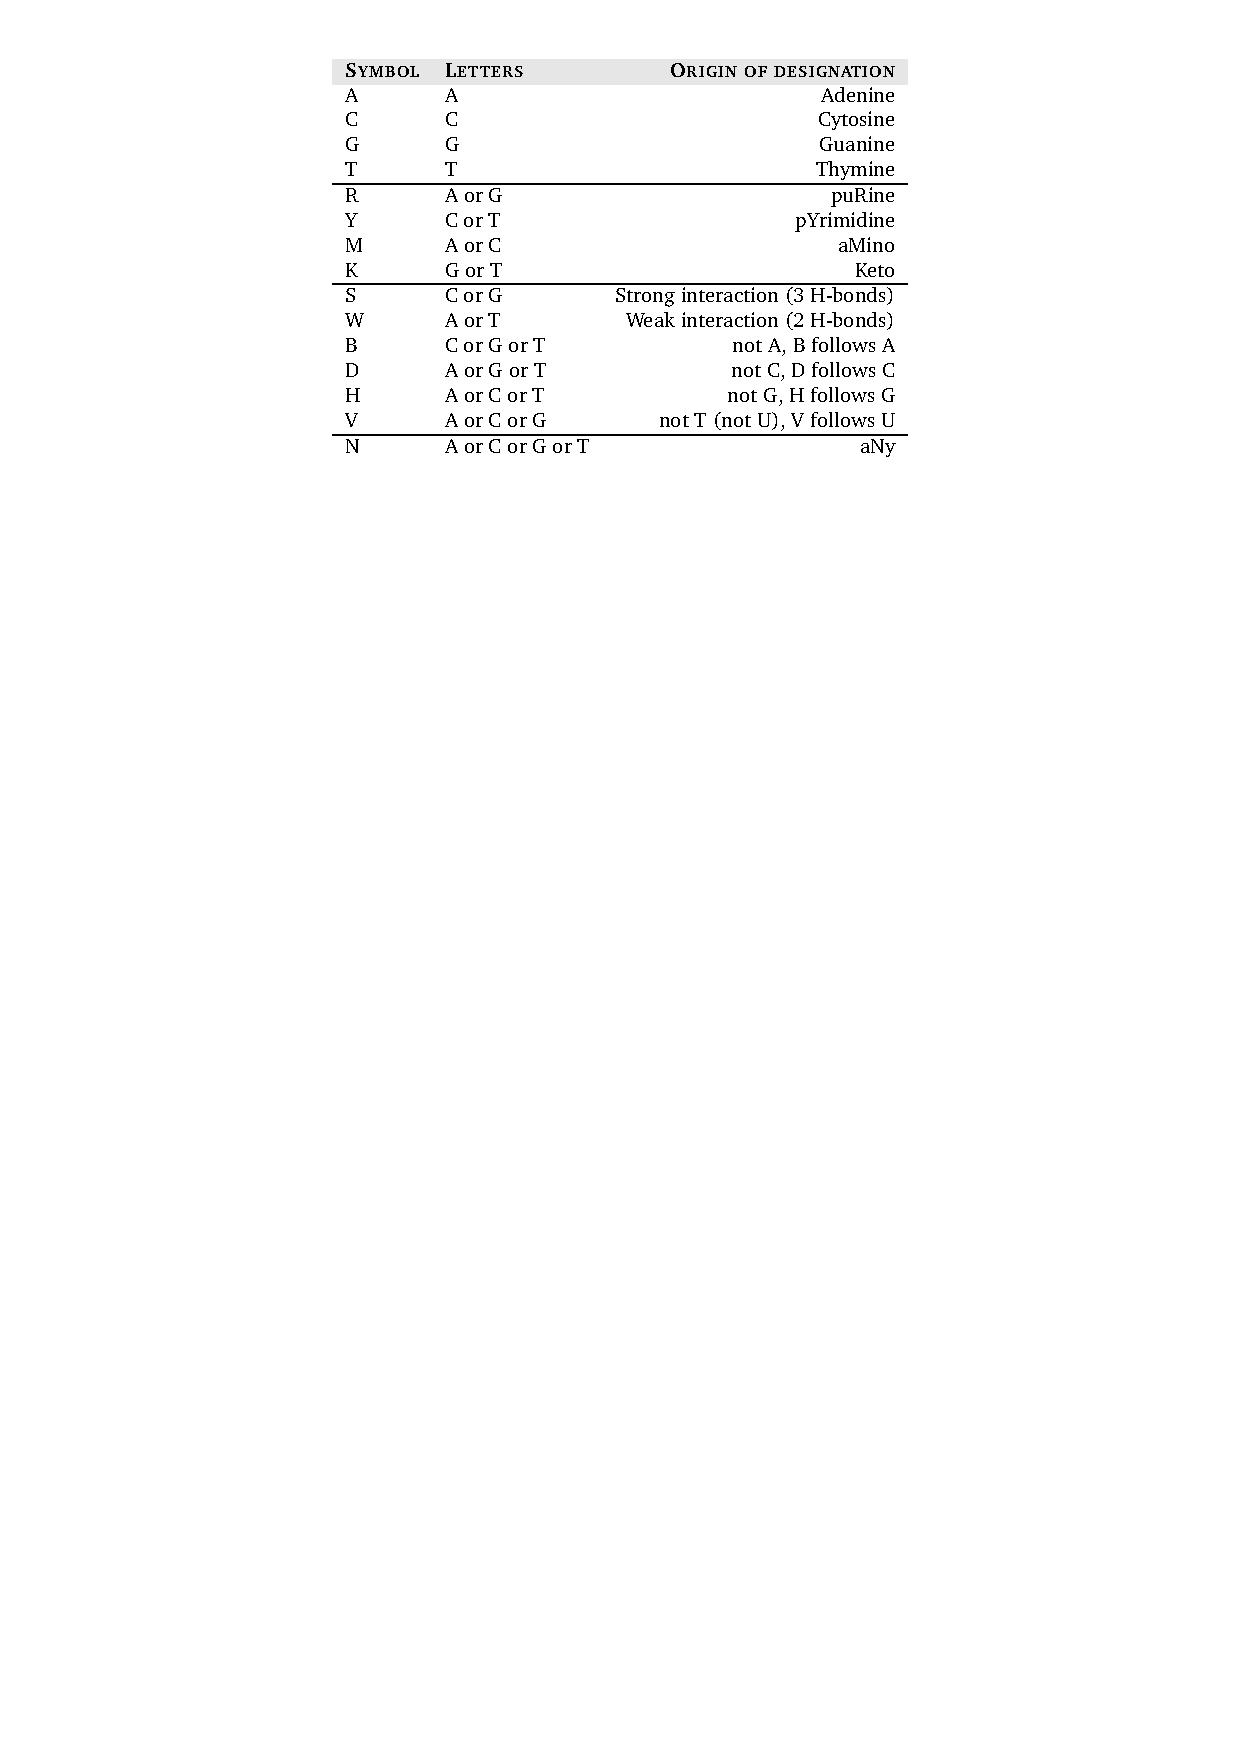
\includegraphics[bb=155 621 498 815,clip]{tables/code1}
\end{minipage}
\mycaption{tab:code1}% label
          {The IUPAC extended genetic alphabet}% lof
          {The IUPAC extended genetic alphabet.}% caption header
          {}
\end{center}
\end{table}


\subsubsectionblue{The number of alignments}

The number of possible alignments between two sequences of $n$ symbols can be computed with the 
following function \citep{waterman:1984a,waterman:1995a}:
\index{alignment!nalns@number of}

\begin{center}
\fcolorbox{white}{verylightgreen}{
\begin{minipage}[][][c]{0.95\linewidth}
\begin{equation}
g(n) \sim \frac{2^{2n}}{4\sqrt{n\pi}}.
\end{equation}
\end{minipage}}
\end{center}

For two sequences of $1,000$ nucleotides, $g(n) > 10{^{600}}$. As direct examination of all these 
alignments is in practice impossible, computational approaches are therefore essential to calculate 
the optimal alignment without exploring all of the combinations.

%%%%
% Table 2: AA alphabet
%%%%
\begin{table}[t!]
\begin{center}
\begin{minipage}{0.4\linewidth}\setlength{\parindent}{0pt}
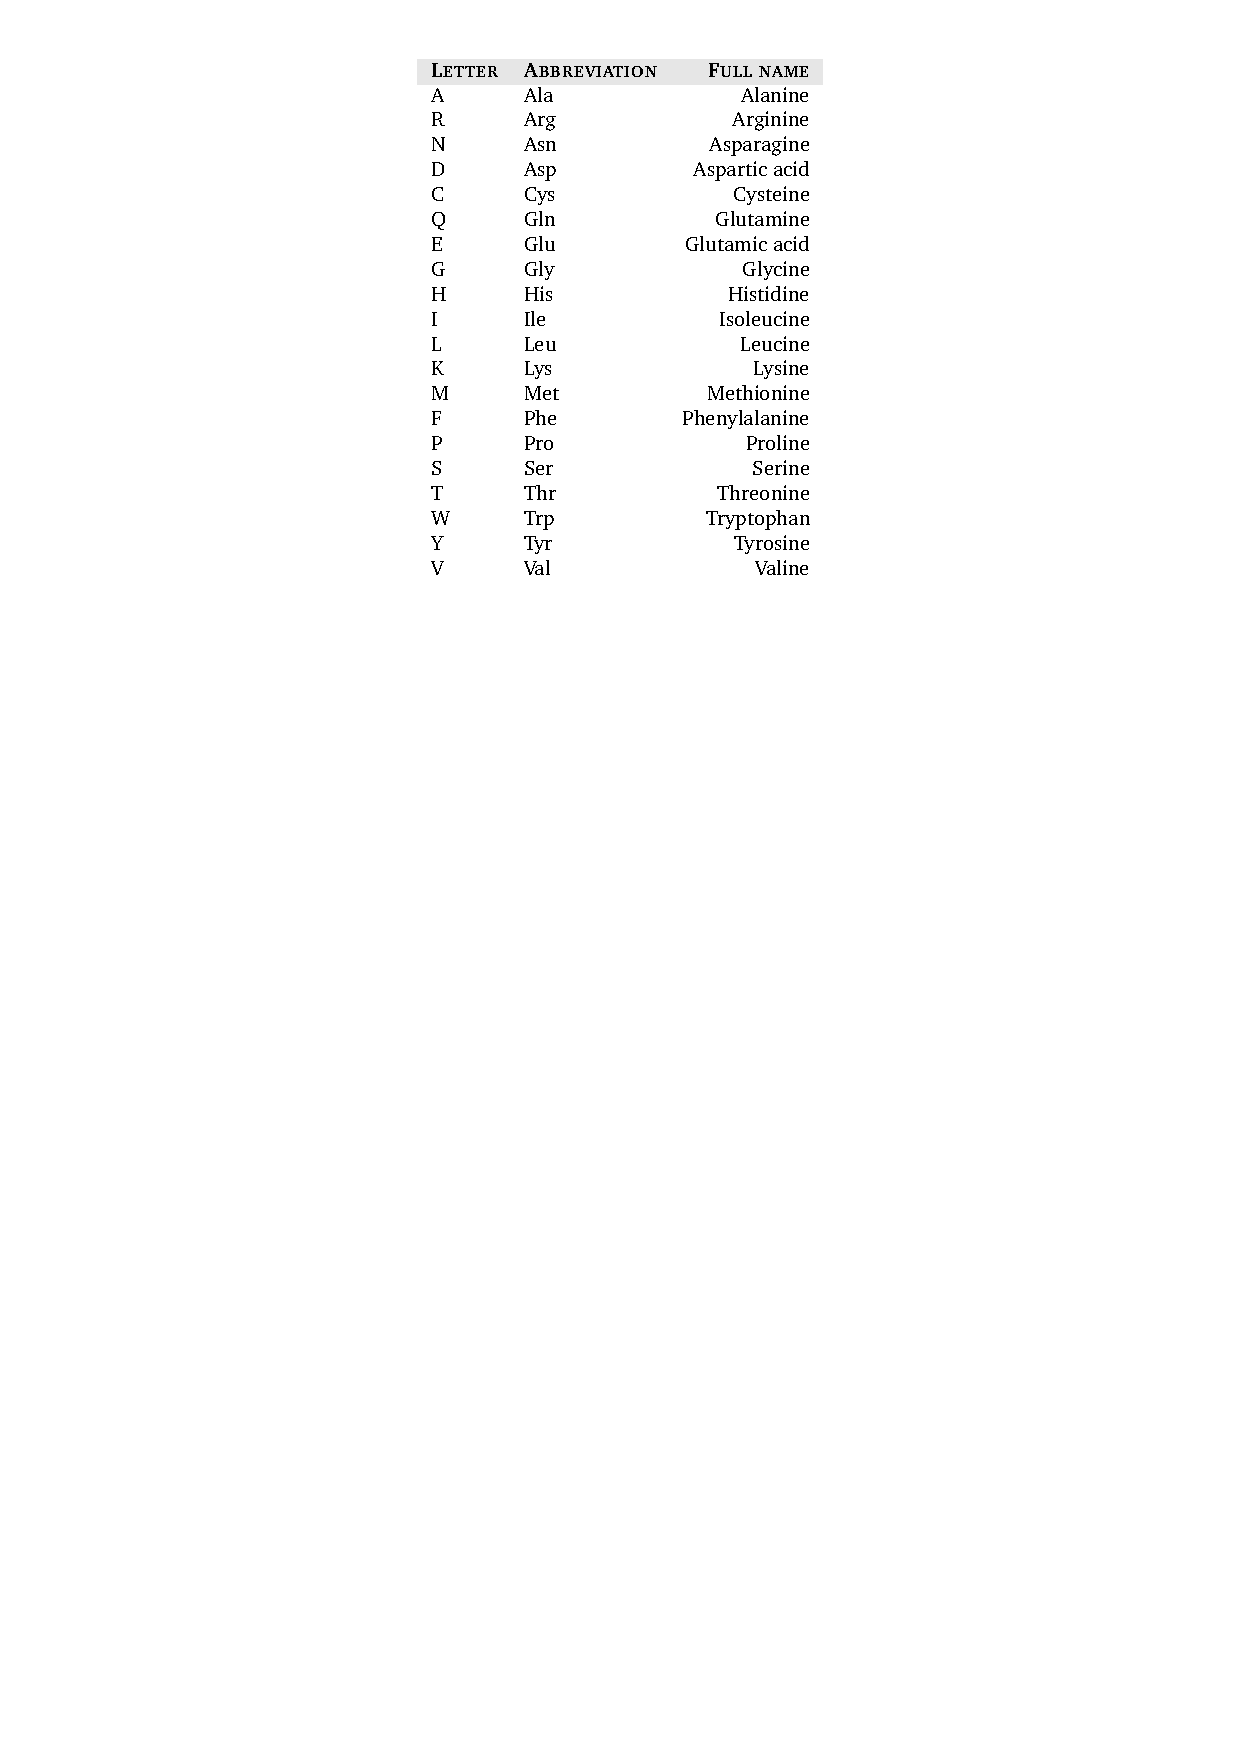
\includegraphics[bb=200 564 397 817,clip]{tables/code2}
\end{minipage}
\mycaption{tab:code2}% label
          {The amino acid alphabet}% lof
          {The amino acid alphabet.}% caption header
          {}
\end{center}
\end{table}

\subsectionblue{Classes of sequence alignments}\label{subsec:classes}
\index{alignment!class@classes}
According to the type of comparison that must be performed between sequences, sequence alignments can 
classified as \citep{mount:2001a}:

\begin{mitemize}
\item
Global alignments: \index{alignment!glob@global}
the entire sequence length must be aligned to include the maximum number of matches. 
Sequences that are quite similar and approximately have the same length are good candidates for global alignment.
\begin{center}
\fcolorbox{white}{verylightgreen}{
\begin{minipage}[][][c]{0.95\linewidth}
\begin{center}
\begin{tabular}{ccccccccccccccccccc}
L & G & P & S & S & K & Q & T & G & K & G & S & -- & S & R & I & W & D & N\\ 
| & & & & & | & & & | & | & | & & & & | & & & | & \\
L & N & -- & I & T & K & S & A & G & K & G & A & I & M & R & L & G & D & A\\
\end{tabular}
\end{center}
\end{minipage}}
\end{center}

\item
Local alignments: \index{alignment!loc@local}
only the stretches of the sequences with the highest density of matches are aligned.
Sequences that differ in length or that only share certain regions are suitable candidates
for local alignment.

\begin{center}
\fcolorbox{white}{verylightgreen}{
\begin{minipage}[][][c]{0.95\linewidth}
\begin{center}
\begin{tabular}{ccccccccccccccccccc}
-- & -- & -- & -- & -- & -- & -- & T & G & K & G & -- & -- & -- & -- & -- & -- & -- & --\\ 
 & & & & & & & & | & | & | & & & & & & & & \\
-- & -- & -- & -- & -- & -- & -- & A & G & K & G & -- & -- & -- & -- & -- & -- & -- & --\\
\end{tabular}
\end{center}
\end{minipage}}
\end{center}
\end{mitemize}

When the number of sequences is two, such alignments receive the name of pairwise alignments
\index{alignment!paraln@pairwise}
as the examples above. If the number of input sequences is higher, they are called multiple sequence
alignments:\index{alignment!mul@multiple}

\begin{mitemize}
\item
Global multiple alignments: the whole set of sequences is aligned at their entire length.
Simply known as multiple alignments, they are the starting point for evolutionary modeling. Each 
column of the alignment is examined and significant changes observed in this position collaborate 
in the construction of a phylogenetic tree. 
\begin{center}
\fcolorbox{white}{verylightgreen}{
\begin{minipage}[][][c]{0.95\linewidth}
\begin{center}
\begin{tabular}{ccccccccccccccccccc}
L & G & P & S & S & K & Q & T & G & K & G & S & -- & S & R & I & W & D & N\\ 
| & & & & & & & & | & | &  & & & &  & & & | & \\
L & N & -- & I & T & K & S & A & G & K & G & A & I & M & R & L & G & D & A\\
| &  & & & & & & & | & | &  & & & & & & & | & \\
L & N & -- & K & Q & Q & S & A & G & K & C & A & I & M & -- & L & G & D & A\\
\end{tabular}
\end{center}
\end{minipage}}
\end{center}

\item
Local multiple alignments: they are equivalent to searching a pattern conserved in a set of sequences.
Rather than be defined as a form of alignment, it is conceptually considered a pattern discovery 
problem.

\begin{center}
\fcolorbox{white}{verylightgreen}{
\begin{minipage}[][][c]{0.95\linewidth}
\begin{center}
\begin{tabular}{ccccccccccccccccccc}
-- & -- & -- & -- & -- & -- & -- & T & G & K & G & -- & -- & -- & -- & -- & -- & -- & --\\ 
-- & -- & -- & -- & -- & -- & -- & A & G & K & G & -- & -- & -- & -- & -- & -- & -- & --\\
-- & -- & -- & -- & -- & -- & -- & A & G & K & C & -- & -- & -- & -- & -- & -- & -- & --\\
\end{tabular}
\end{center}
\end{minipage}}
\end{center}
\end{mitemize}


\sectionorange{An anthology of algorithms for global alignments}\label{sec:global}

This section aims to be a catalogue of different approaches to solve the global pairwise alignment which
was the first problem introduced in the field of sequence comparisons. Naturally, the extension to the
multiple alignment of sequences has been also treated although optimal solutions were discarded because of 
their expensive time and space costs. Different heuristics to cope with multiple alignment are explained 
in detail in Section \ref{sec:msa}.

\subsectionblue{The Needleman and Wunsch algorithm (1970)}\label{nw}

\index{algorithms!nw@Needleman and Wunsch} \index{alignment!nw@Needleman and Wunsch}
For the authors, the similarity or maximum match value between two proteins depends on the largest number
of amino acids from the first protein that can be matched with those of the second one allowing possible 
interruptions in either sequence. 

Each pair of amino acids from each sequence is the smallest unit of significance. All possible pair 
combinations are represented in a two-dimensional matrix $M$. The pathways through the cells of the 
matrix are representations of every possible comparison of the two sequences. If a given value is 
assigned to each identity and mismatch, the maximum match between two sequences $A$ and $B$ is then 
the largest number that would result from the sum of the cell values of every pathway.

The original \citeauthor{needleman:1970a} algorithm is actually a description of a method to 
systematically count the number of identities (denoted as 1's in the simplest formulation) between both 
sequences. No complexity analysis was provided although a careful analysis determines the cost of the
process is cubic (see next section). In addition, the authors implicitly suggested the extension of 
the method to allow multiple comparison of several proteins or the inclusion of a gap penalty factor as 
a function depending on the length of the gap.

The assessment of the significance of a given match value was also proposed: first, two sets of random 
sequences with the same composition of the original proteins are constructed; second, the maximum-match 
between pairs of these sequences is determined several times and is compared to the value obtained between 
real proteins; third, the match between one of the real proteins and several of the random sequences 
is also computed and evaluated. In all of the cases, the difference between the real match and the 
artificial ones should be statistically significant. Otherwise, the match between both proteins would be 
explained in part only by a similar composition.

%%%%
% Figure 2: N-W Matrix (figure 1 paper)
%%%%
\begin{figure}[t!]
\begin{center}
\setlength{\fboxsep}{0pt}
%\fbox{
\incgraph{width=0.4\linewidth}{ps/nw}%}
\mycaption{fig:nw}% label
          {The maximum-match operation for necessary pathways}% lof
          {The maximum-match operation for necessary pathways.}% caption header
          {The cell $(R,R,1)$ corresponds to the current $M(i,j)$. Adapted from \citet{needleman:1970a}.}
\end{center}
\end{figure}

\subsubsectionblue{Formulation and cost}

The objective of the algorithm is to compute the pathway in the matrix $M$ that according to a certain
scoring schema is assigned the maximum value. The procedure to efficiently compute this value consists 
of two stages (see Figure \ref{fig:nw}):
\begin{menumerate}
\item
Each cell of the matrix $M(i,j)$ is assigned the corresponding value whether there is a match or a 
mismatch in this position (e.g. $1$ for identities, void or $0$ for mismatches).
\item
Beginning at the terminals of the sequences and proceeding toward the origins in the matrix, the value 
of the maximum-match starting at each cell $M(i,j)$ can be obtained by adding to its value, the maximum
value from among all the cells which lie on a pathway to it. The pathways are negatively weighted with the 
value $g$ according to the number of gaps they contain. 
\end{menumerate}

\begin{center}
\fcolorbox{white}{verylightgreen}{
\begin{minipage}[][][c]{0.95\linewidth}
\begin{equation}
M(i,j) = M(i,j) +
max
\left\{
\begin{array}{lr}
M(i+1,j+1) &\\
M(i',j+1) + g \times (i' -i + 1),& i+2 \leq i' \leq |A| \\
M(i+1,j') + g \times (j' -j + 1),& j+2 \leq j' \leq |B|. \\
\end{array}\right.
\end{equation}
\end{minipage}}
\end{center}

If $|A| = |B| = n$, then the cost of visiting each cell of the matrix is $O(n^2)$. Additionally, for 
each cell the best pathway among all of the possible ones in the previous row, in the previous column 
and in the diagonal is searched. The cost of accessing the values of the pathways in a given column or 
row is $O(n)$, while accessing the diagonal is constant $O(1)$. Therefore, the final cost of the 
\citeauthor{needleman:1970a} algorithm is $O(n^3)$.

\subsubsectionblue{Implementation}

The implementation of the algorithm is shown in Figure \ref{fig:nwalg}. The matrix is processed
following a systematic order. Both processing steps described above are integrated in a single 
one. For each pair of amino acids from both sequences represented by a cell $M(i,j)$ in the matrix , the 
optimal pathway starting there is constructed selecting the best pathway in the diagonal, and in the 
$i+1$ row and the $j+1$ column (here weighting according to the number of gaps) that have been 
previously computed.

The matrix $P$ is used to record the cell from which the maximum pathway was selected. The retrievement 
of the solution, not shown here, consists on (1) searching the maximum value (cell $x,y$) both in the first 
row and in the first column and (2) using recursively the coordinates in $P(x,y)$, to construct the 
arrangement of both sequences until a cell at the last column or row is reached.


\subsectionblue{The Sellers algorithm (1974)}\label{sellers}

\index{algorithms!sellers@Sellers} \index{alignment!selal@Sellers}
In the 1970s, most techniques used in taxonomic tree construction depended on the introduction
of a measure of distance between sequences \citep{fitch:1967a}. The work on distances or metrics on
protein sequences was essentially based on discovering what genetic mutations were required to change
one sequence into another.

\clearpage
A metric space is a function $\rho: S \times S \rightarrow \mathcal{Z^+}$ on a generic set $S$, with 
the following properties:

\begin{center}
\fcolorbox{white}{verylightgreen}{
\begin{minipage}[][][c]{0.95\linewidth}
\begin{center}
\begin{tabular}{ll}
\emph{Non-negative} & $\forall a,b \in S: \rho(a,b) \geq 0$\\
\emph{Identity} & $\forall a,b \in S: \rho(a,b) = 0 \Leftrightarrow a = b$\\
\emph{Reflexivity} & $\forall a,b \in S: \rho(a,b) = \rho(b,a)$\\
\emph{Transitivity} & $\forall a,b,c \in S: \rho(a,b) \leq \rho(a,c) + \rho(c,b)$.\\
\end{tabular}
\end{center}
\end{minipage}}
\end{center}

\citet{sellers:1974a} described the construction of an evolutionary tree, which assumes that evolutionary
distance is a metric. The minimum distance $D(A,B)$ between two sequences $A$ and $B$ is defined as the 
smallest possible weighted sum of insertions, deletions, and substitutions which transforms one sequence
into the other.

\citeauthor{sellers:1974a} showed that if a scoring function $d(a,b)$\footnote{Also known as a weighting 
scheme.} forms a metric space over the underlying alphabet of symbols then the minimum distance function 
$D(A,B)$ forms a metric space over the set of finite sequences constructed with such an alphabet. In 
addition, he proportioned the dynamic programming recurrence to efficiently compute the minimum distance $D$
between two sequences using several scoring functions. In fact, many comparison algorithms that use 
distance functions with a given weighting scheme provide an optimal alignment only if such a scheme is a 
metric \citep{tyler:1991a}.


%%%%
% Figure 3: N-W algorithm
%%%%
\begin{figure}[t!]
\begin{center}
\scalebox{1}{
\fcolorbox{white}{verylightgreen}{
\begin{minipage}[][][c]{0.95\linewidth}
\begin{algorithmic}[5]
\REQUIRE $A,B$: sequences; id,mis,gap $\in \mathcal{Z}$
\STATE
\STATE \COMMENT{Begin the series of sums from last row and column}
\FOR{$i=|A|$ to $1$}
\FOR{$j=|B|$ to $1$}
\STATE \COMMENT{Setting the identity or mismatch value for the cell}
\IF{$a_i = b_j$}
\STATE $M(i,j) \leftarrow$ id;
\ELSE
\STATE $M(i,j) \leftarrow$ mis;
\ENDIF
\IF{$i \neq |A|$ and $j \neq |B|$}
\STATE \COMMENT{Search the maximum-match pathway beginning here}
\STATE \COMMENT{A. The maximum from diagonal}
\STATE max $\leftarrow M(i+1,j+1)$;
\STATE $P(i,j) \leftarrow (i+1,j+1)$;
\STATE \COMMENT{B. The maximum value from previous column}
\STATE ngaps $\leftarrow 1$;
\FOR{$i'= i + 2$ to $|A|$}
\STATE value $\leftarrow M(i',j+1) + \mbox{gap * ngaps}$; 
\IF{value $> \mbox{max}$}
\STATE max $\leftarrow$ value;
\STATE $P(i,j) \leftarrow (i',j+1)$;
\ENDIF
\STATE ngaps $\leftarrow$ ngaps + 1;
\ENDFOR
\STATE \COMMENT{C. The maximum value from previous row}
\STATE ngaps $\leftarrow 1$;
\FOR{$j'= j + 2$ to $|B|$}
\STATE value $\leftarrow M(i+1,j') + \mbox{gap * ngaps}$;
\IF{value $> \mbox{max}$}
\STATE max $\leftarrow $ value;
\STATE $P(i,j) \leftarrow (i+1,j')$;
\ENDIF
\STATE ngaps $\leftarrow$ ngaps + 1;
\ENDFOR
\STATE \COMMENT{The maximum-match pathway is formed}
\STATE $M(i,j) \leftarrow M(i,j) + \mbox{max}$;
\ENDIF
\ENDFOR
\ENDFOR
\end{algorithmic}
\end{minipage}}}
\mycaption{fig:nwalg}% label
          {The \citeauthor{needleman:1970a} algorithm}% lof
          {The \citeauthor{needleman:1970a} algorithm.}% caption header
          {}
\end{center}
\end{figure}


\subsubsectionblue{Formulation and cost}

\citeauthor{sellers:1974a} generalized the algorithm to allow for various weighting schemes. Let $a$ and $b$ be two
symbols. The simplest scheme $d$ to score this match is defined as:

\begin{center}
\fcolorbox{white}{verylightgreen}{
\begin{minipage}[][][c]{0.95\linewidth}
\begin{equation}
d(a,b) = 
\left\{
\begin{array}{lr}
0 & \mbox{if}~~a = b\\
1 & \mbox{if}~~a \neq b.\\
\end{array}\right.
\end{equation}
\end{minipage}}
\end{center}

Using this scoring function $d$, the following recurrence calculates the optimal distance between two
sequences $A = (a_1, a_2, \ldots a_m)$ and $B = (b_1, b_2, \ldots b_n)$, and provides the initial values as well:

\begin{center}
\fcolorbox{white}{verylightgreen}{
\begin{minipage}[][][c]{0.95\linewidth}
\begin{equation}
\begin{array}{ll}
D(i,j) = &
min \left\{
\begin{array}{ll}
D(i-1,j-1) + d(a_i,b_j) & \mbox{\emph{Match}}\\
D(i-1,j) + d(a_i,-) & \mbox{\emph{Gap in $B$}}\\
D(i,j-1) + d(-,b_j) & \mbox{\emph{Gap in $A$}}\\
\end{array}\right. ,\\[0.75cm]

D(i,0) = & \sum_{k=0}^{i}{d(a_k,-)},\\
D(0,j) = & \sum_{k=0}^{j}{d(-,b_k)}.
\end{array}
\label{eq:sellers}
\end{equation}
\end{minipage}}
\end{center}

To avoid the exponential number of combinations to construct an alignment between two sequences, this
dynamic programming recurrence decompose the problem in smaller alignments of prefixes of the original
sequences. Thus, starting from the one-letter prefixes , the minimum distance of the alignment 
ending at the prefixes $A_{1,i}$ and $B_{1,j}$ can be calculated from the three different forms of finishing
such an alignment:

\begin{center}
\fcolorbox{white}{verylightgreen}{
\begin{minipage}[][][c]{0.95\linewidth}
\begin{center}
%\scalebox{0.7}{
%\begin{minipage}[][][c]{1.25\linewidth}
\begin{tabular}{ccc}
\fbox{\begin{tabular}{lllll}
$\bullet$ & $\bullet$ & $\bullet$ & $\bullet$ & $a_i$\\
$\bullet$ & $\bullet$ & $\bullet$ & $\bullet$ & $b_j$\\
\end{tabular}}
&
\fbox{\begin{tabular}{lllll}
$\bullet$ & $\bullet$ & $\bullet$ & $\bullet$ & $a_i$\\
$\bullet$ & $\bullet$ & $\bullet$ & $\bullet$ & --\\
\end{tabular}}
&
\fbox{\begin{tabular}{lllll}
$\bullet$ & $\bullet$ & $\bullet$ & $\bullet$ & --\\
$\bullet$ & $\bullet$ & $\bullet$ & $\bullet$ & $b_j$\\
\end{tabular}}\\
Match & Ins in $A$, Del in $B$ & Del in $A$, Ins in $B$.\\
\end{tabular}
%\end{minipage}}
\end{center}
\end{minipage}}
\end{center}

%%%%
% Figure 4: DProgramming Matrix
%%%%
\begin{figure}[t!]
\begin{center}
\setlength{\fboxsep}{0pt}
%\fbox{
\incgraph{width=0.6\linewidth}{ps/dp}%}
\mycaption{fig:dp}% label
          {The dynamic programming matrix}% lof
          {The dynamic programming matrix.}% caption header
          {In yellow, the part of the alignment matrix that has been computed. In blue, the part that must be still calculated. The cell $D(i,j)$ is the match currently in process.}
\end{center}
\end{figure}

If both sequences have the same length $n$, the cost of the \citeauthor{sellers:1974a} algorithm is 
$O(n^2)$ which is the time to visit all of the cells of the dynamic programming matrix (see Figure 
\ref{fig:dp}). For each cell, only three neighbours are consulted: in the diagonal, in the horizontal
and in the vertical.

The procedure to trace-back the distance matrix, reconstructing the alignment was adapted from
\citeauthor{needleman:1970a} by \citeauthor{sellers:1974a}. A second matrix of pointers is needed for 
recording from which direction was taken the value to update a given cell matrix.

\subsubsectionblue{Implementation}

The \citeauthor{sellers:1974a} algorithm requires to fit the \citeauthor{needleman:1970a} $m \times n$
matrix in an artificial 0-column and 0-row to increase the initial distance when starting the alignment 
with gaps\footnote{There is an easy modification of the algorithm to permit not to punish this kind of 
gaps.}. 

Then, the algorithm starts at $D(1,1)$ and the matrix is filled by rows (from top to bottom) and within a 
row by columns (from left to right). Thus, when a cell $D(i,j)$ is reached, its neigbours $D(i-1,j-1)$, 
$D(i-1,j)$ and $D(i,j-1)$ have been already calculated.

%%%%
% Figure 5: Sellers algorithm
%%%%
\begin{figure}[t!]
\begin{center}
\scalebox{1}{
\fcolorbox{white}{verylightgreen}{
\begin{minipage}[][][c]{0.95\linewidth}
\begin{algorithmic}[5]
\REQUIRE $A,B$: sequences;  $d$: metric on $\Sigma$
\STATE
\STATE \COMMENT{Initialize the 0-column and the 0-row}
\FOR{$i=0$ to $|A|$}
\STATE $D(i,0) \leftarrow i \times d(a_i,-)$;
\ENDFOR
\FOR{$j=1$ to $|B|$}
\STATE $D(0,j) \leftarrow j \times d(b_j,-)$;
\ENDFOR
\STATE \COMMENT{Filling the matrix}
\FOR{$i=1$ to $|A|$}
\FOR{$j=1$ to $|B|$}
\STATE \COMMENT{A. Match}
\STATE min $\leftarrow D(i-1,j-1) + d(a_i,b_j)$;
\STATE $P(i,j) \leftarrow (i-1,j-1)$;
\STATE \COMMENT{B. Gap in sequence $B$}
\STATE value $\leftarrow D(i-1,j) + d(a_i,-)$;
\IF{value $<$ min}
\STATE min $\leftarrow$ value;
\STATE $P(i,j) \leftarrow (i-1,j)$;
\ENDIF
\STATE \COMMENT{C. Gap in sequence $A$}
\STATE value $\leftarrow D(i,j-1) + d(-,b_j)$;
\IF{value $<$ min}
\STATE min $\leftarrow$ value;
\STATE $P(i,j) \leftarrow (i,j-1)$;
\ENDIF
\STATE $D(i,j) \leftarrow$ min;
\ENDFOR
\ENDFOR
\end{algorithmic}
\end{minipage}}}
\mycaption{fig:sellersalg}% label
          {The \citeauthor{sellers:1974a} algorithm}% lof
          {The \citeauthor{sellers:1974a} algorithm.}% caption header
          {}
\end{center}
\end{figure}

Contrarily to the \citeauthor{needleman:1970a} algorithm (in which the maximum match was searched in the 
last column and the last row), the minimum distance between both sequences will be saved at the end into 
the cell $D(m,n)$ because of the different initialization.

As in the case of the \citeauthor{needleman:1970a}, there is an auxiliary matrix $P$ that saves the 
source of each calculation in a given cell to recursively reconstruct the alignment with such a distance.

\subsectionblue{A linear space algorithm: Hirschberg (1975)}\label{linearspace}

\index{algorithms!hirs@Hirschberg} \index{alignment!hirsal@Hirschberg}
In some occasions when aligning two sequences, the limiting factor is not the time but the space (memory).
Any algorithm that solves the alignment of two sequences can not decrease the quadratic time cost unless
any assumption is made over the length of the inputs. However, the quadratic cost in terms of space can 
be reduced to a linear cost.

\citet{hirschberg:1975a} designed a divide and conquer algorithm to solve the LCS problem in linear space
without increasing the asymptotic time cost. Later, \citet{myers:1988a} demonstrated how this technique
could optimally deal with general sequence alignment problems.

The key point of the algorithm is based on the fact that in the alignment between the sequences $A$ and
$B$, any element of $A$ will be aligned either to a gap or another element in $B$. Thus, the problem
of aligning both sequences can be expressed in terms of making this decision for a current element $a_i$,
assuming the optimal alignments between the subsequences from $A$ and $B$ around this element are already 
computed.

Another important fact is the ability to compute the distance between two sequences in linear space.
If the dynamic programming matrix is filled in from top to bottom (row by row), and fixing a row, from
left to right (column by column), then the values in a row $i$ depend only on the values stored at the 
previous row $i-1$ and on the values in the same row $i$. The other previous rows are therefore not necessary
to obtain the final value $D(m,n)$ \citep{myers:1991a,meidanis:1997a}.

Furthermore, instead of using two arrays to represent the rows $i$ and $i+1$, the computation can be 
performed in a single array $D$ (see Figure \ref{fig:twoarray} (A)), overwriting the old values on the left 
of the current column $j$. The equivalence between each cell $D(i,j)$ in the original dynamic programming matrix 
and the content of this unidimensional array $D$ when the row $i$ is being processed is:

\begin{center}
\fcolorbox{white}{verylightgreen}{
\begin{minipage}[][][c]{0.95\linewidth}
\begin{equation}
\begin{array}{l}
D(k) \approx D(i,k) ~~\mbox{when}~~ k < j ~~\mbox{(current row, $i$)}\\
D(k) \approx D(i-1,k) ~~\mbox{when}~~ k \geq j ~~\mbox{(previous row, $i-1$)}.\\
\end{array}
\end{equation}
\end{minipage}}
\end{center}

%%%%
% Figure 6: Using an array to compute D(i,j)
%%%%
\begin{figure}[t!]
\begin{center}
\setlength{\fboxsep}{0pt}
\begin{tabular}{ccc}
%\hline
%\hline
\incgraph{width=4cm,height=4cm}{ps/hir1} &
\incgraph{width=4cm,height=4cm}{ps/hir2} &
\incgraph{width=4cm,height=4cm}{ps/hir3}\\
%\hline
A & B & C
\end{tabular}
\mycaption{fig:twoarray}% label
          {The \citeauthor{hirschberg:1975a} linear space approach}% lof
          {The \citeauthor{hirschberg:1975a} linear space approach.}% caption header
          {(A) Using a single array to compute $D(i,j)$. (B) The divide and conquer strategy applied over the dynamic programming approach. (C) The backward propagation of values.}
\end{center}
\end{figure}

\subsubsectionblue{Formulation and cost}

In the optimal alignment between two sequences $A$ and $B$, a given element $a_i$ from $A$ will be either
matched to another element $b_j$ from $B$ or aligned to a gap between a certain $b_j$ and $b_{j+1}$. Then,
this optimal alignment can be decomposed in three parts:

\begin{menumerate}
\item
The optimal alignment between the elements from both sequences on the left (prefixes).
\item
The match between $a_i$ with a certain $b_j$ or a gap.
\item
The optimal alignment between the elements from both sequences on the right (suffixes).
\end{menumerate}

For a given $i$, the optimal point $j$ can be unveiled with the application of the algorithm to compute 
only the distance between two sequences in linear space time. Such a solution provides the point in 
which the optimal alignment path will cross the $i$-row in the the dynamic programming matrix. As it is 
shown in Figure \ref{fig:twoarray} (B), once the points $i$ and $j$ are established, the general 
problem is divided into two subproblems and recursively the same procedure is applied until reaching the 
base case (empty sequences).

The algorithm that computes only the distance between two sequences in linear space is in fact a method
to provide the minimum distance between the first sequence and any of the prefixes of the second sequence. 
As the right parts are also aligned in the main procedure, a modification of such an algorithm is 
necessary to obtain the minimum distance between the first sequence and any of the suffixes of the second 
one.

In fact, the dynamic programming scheme is not restricted to construct the final alignment from 
alignments between prefixes of the input sequences. The same recurrence is appropriate for building it
from alignments between suffixes of them. The procedure now begins in the position $D(|A|,|B|)$, and
propagates the values from bottom to top, and from right to left (see Figure \ref{fig:twoarray} (C)). 
The Equation \ref{eq:sellers} must be slightly modified to accommodate this backward propagation:

\begin{center}
\fcolorbox{white}{verylightgreen}{
\begin{minipage}[][][c]{0.95\linewidth}
\begin{equation}
\begin{array}{ll}
D(i,j) = &
min \left\{
\begin{array}{ll}
D(i+1,j+1) + d(a_i,b_j) & \mbox{\emph{Match}}\\
D(i+1,j) + d(a_i,-) & \mbox{\emph{Gap in $B$}}\\
D(i,j+1) + d(-,b_j) & \mbox{\emph{Gap in $A$}}\\
\end{array}\right. ,\\[0.75cm]

D(i,|B|+1) = & \sum_{k=0}^{i}{d(a_k,-)},\\
D(|A|+1,j) = & \sum_{k=0}^{j}{d(-,b_k)}.\\
\end{array}
\end{equation}
\end{minipage}}
\end{center}

The cost of obtaining just the value $D(i,j)$ following the forward or the backward manner is again 
quadratic in terms of time. However, the cost in terms of space of this function is linear as 
only a single array is used in both cases.

To compute the cost of a recursive divide and conquer function, a different cost scheme must be applied.
Let us consider $n$ the length of both input sequences that are aligned. At the beginning, the routine
performs some computations and then, there is an approximate $\frac{n}{2}$ reduction in the size of the 
input data for the subsequent two recursive calls. The cost $T(n)$ of computing such a recursive function 
can be expressed in terms of its children as:

\begin{center}
\fcolorbox{white}{verylightgreen}{
\begin{minipage}[][][c]{0.95\linewidth}
\begin{equation}
\begin{array}{l}
T(n) = 
\left\{
\begin{array}{lll}
g(n) & 0 \leq n < c & \mbox{\emph{Base case}}\\
a T(\frac{n}{c}) + b n^k & n \geq c & \mbox{\emph{Recursive case}}\\
\end{array}\right.,
\end{array}
\end{equation}
\end{minipage}}
\end{center}

where $a$ is the number of recursive calls, $c$ is the size of the fragmentation and $b n^k$ is the
cost of the non-recurrent operations performed on each call. From the relationship between $a$ and $c^k$, 
the corresponding cost function is inferred following the Master Theorem of recurrent equations (see 
\citet{cormen:2001a}, Sections 4.3 and 4.4). In the \citeauthor{hirschberg:1975a} recurrence is easy to 
notice $g(n) \in O(n)$, $a = 2$, $b = 2$, $c = 2$ and $k = 2$. Therefore as $a<c^k$ or $2<2^2$, according to 
the Master Theorem $T(n) \in \Theta(n^k)$, that is $T(n) \in \Theta(n^2)$. 

Nevertheless, the spatial cost of the \citeauthor{hirschberg:1975a} algorithm is linear. All of the computations 
on the theoretical dynamic programming matrix are performed over single rows implemented with unidimensional
arrays.


%%%%
% Figure 7: Computing D(m,n) in O(n) space: FWD and RVS
%%%%
\begin{figure}[t!]
\begin{center}
\scalebox{0.7}{
\fcolorbox{white}{verylightgreen}{
\begin{tabular}{c|c}
\begin{minipage}[][][c]{0.6\linewidth}
\textbf{Procedure} ComputeOnlyDistanceForward\\[0ex]
\begin{algorithmic}[5]
\REQUIRE $A,B$: sequences;  $d$: metric on $\Sigma$
\ENSURE $D$: array (|B|+1);
\STATE
\STATE \COMMENT{Simulating the initialization of the 0-row}
\FOR{$j=0$ to $|B|$}
\STATE $D(j) \leftarrow j \times d(-,b_j)$;
\ENDFOR
\FOR{$i=1$ to $|A|$}
\STATE \emph{diag} $\leftarrow D(0)$;
\STATE \COMMENT{Simulating the initialization of the i-row}
\STATE $D(0) \leftarrow i \times d(a_i,-)$;
\FOR{$j=1$ to $|B|$}
\STATE \COMMENT{This cell will be the next diagonal}
\STATE \emph{temp} $\leftarrow D(j)$;
\STATE \COMMENT{A. Match ($\nwarrow$)}
\STATE min $\leftarrow$ \emph{diag} $+ d(a_i,b_j)$;
\STATE \COMMENT{B. Gap in sequence $A$ ($\uparrow$)}
\STATE value $\leftarrow D(j) + d(a_i,-)$;
\IF{value $<$ min}
\STATE min $\leftarrow$ value;
\ENDIF
\STATE \COMMENT{C. Gap in sequence $B$ ($\leftarrow$)}
\STATE value $\leftarrow D(j-1) + d(-,b_j)$;
\IF{value $<$ min}
\STATE min $\leftarrow$ value;
\ENDIF
\STATE $D(j) \leftarrow$ min;
\STATE \COMMENT{Update diagonal}
\STATE \emph{diag} $\leftarrow$ \emph{temp}
\ENDFOR
\ENDFOR
\end{algorithmic}
\end{minipage}
& % second column
\begin{minipage}[][][c]{0.6\linewidth}
\textbf{Procedure} ComputeOnlyDistanceBackward\\[0ex]
\begin{algorithmic}[5]
\REQUIRE $A,B$: sequences;  $d$: metric on $\Sigma$
\ENSURE $D$: array (|B|+1);
\STATE
\STATE \COMMENT{Simulating the initialization of the last row}
\FOR{$j=|B|$ to $1$}
\STATE $D(j) \leftarrow j \times d(-,b_j)$;
\ENDFOR
\FOR{$i=|A|-1$ to $1$}
\STATE \emph{diag} $\leftarrow D(|B|+1)$;
\STATE \COMMENT{Simulating the initialization of the i-row}
\STATE $D(|B|+1) \leftarrow i \times d(a_i,-)$;
\FOR{$j=|B|$ to $1$}
\STATE \COMMENT{This cell will be the next diagonal}
\STATE \emph{temp} $\leftarrow D(j)$;
\STATE \COMMENT{A. Match ($\nwarrow$)}
\STATE min $\leftarrow$ \emph{diag} $+ d(a_i,b_j)$;
\STATE \COMMENT{B. Gap in sequence $A$ ($\downarrow$)}
\STATE value $\leftarrow D(j) + d(a_i,-)$;
\IF{value $<$ min}
\STATE min $\leftarrow$ value;
\ENDIF
\STATE \COMMENT{C. Gap in sequence $B$ ($\rightarrow$)}
\STATE value $\leftarrow D(j+1) + d(-,b_j)$;
\IF{value $<$ min}
\STATE min $\leftarrow$ value;
\ENDIF
\STATE $D(j) \leftarrow$ min;
\STATE \COMMENT{Update diagonal}
\STATE \emph{diag} $\leftarrow$ \emph{temp}
\ENDFOR
\ENDFOR
\end{algorithmic}
\end{minipage}
\end{tabular}}}
\mycaption{fig:cdistance}% label
          {An algorithm to compute $D(i,j)$ in $O(n)$ space cost}% lof
          {An algorithm to compute $D(i,j)$ in $O(n)$ space cost.}% caption header
          {(Left) The computation is done from $D(0,0)$ to $D(|A|,|B|)$. (Right) The 
           computation is done from $D(|A|+1,|B|+1)$ to $D(1,1)$.}
\end{center}
\end{figure}

\subsubsectionblue{Implementation}

\subsubsectionblue{Computing the value $D(i,j)$ in linear space}

To implement the fusion of the previous row and the current one in a single array in a forward manner, 
the temporary variables \emph{diag} and \emph{temp} are necessary to save the values $D(i-1,j-1)$ 
--diagonal-- and $D(i-1,j)$ --gap in $A$--, respectively. At the end of the forward computation,
the array $D$ will contain the same values as the last row of the bidimensional classic dynamic 
programming matrix, that is, the distance between the sequence $A$ and any of the prefixes of the sequence
$B$. In particular, the array position $D(|B|)$ will contain the distance between the sequences $|A|$ 
and $|B|$

The backward computation is symmetrical to the forward processing. The propagation of values starts now
in the position $D(|B|+1)$, moving the values from right to left, and from bottom to top. At the end of the
backward computation, the array $D$ will contain the same values as the last row of the bidimensional 
reverse dynamic programming matrix, that is the distance between the sequence $A$ and any of the suffixes
of the sequence $B$. In particular, the array position $D(1)$ will contain the distance between the 
sequences $|A|$ and $|B|$.

%%%%
% Figure 8: The alignment of two sequences in linear space
%%%%
\begin{figure}[t!]
\begin{center}
\scalebox{0.8}{
\fcolorbox{white}{verylightgreen}{
\begin{minipage}[][][c]{0.95\linewidth}
\textbf{Procedure} Alignment\\[0ex]
\begin{algorithmic}[5]
\REQUIRE $A,B$: sequences;  $d$: metric on $\Sigma$; $i_1,i_2,j_1,j_2,al_1,al_2 in ~\mathcal{Z}$
\ENSURE \emph{alA}: array ($al_1 .. al_2$), \emph{alB}: array ($al_1 .. al_2$);
\STATE
\IF{$A_{i_1,i_2} = \emptyset$}
\STATE \COMMENT{Base case 1}
\FOR{$k=j_1 to j_2$}
\STATE \emph{alA}$(al_1+k) \leftarrow -$;
\STATE \emph{alB}$(al_1+k) \leftarrow B(j_1+k)$;
\ENDFOR
\STATE $al_2 \leftarrow al_1 + k$;
\ELSIF{$B_{j_1,j_2} = \emptyset$}
\STATE \COMMENT{Base case 2}
\FOR{$k=i_1$ to $i_2$}
\STATE $alA(al_1+k) \leftarrow A(i_1+k)$;
\STATE $alA(al_1+k) \leftarrow -$;
\ENDFOR
\STATE $al_2 \leftarrow al_1 + k$;
\ELSE
\STATE \COMMENT{General case}
\STATE \COMMENT{Select the point $i$}
\STATE $i \leftarrow \lfloor \frac{i_1+i_2}{2} \rfloor$
\STATE \COMMENT{Compute the distance to the prefixes/suffixes of $B$}
\STATE \emph{prefDist} $\leftarrow$ ComputeOnlyDistanceForward($A_{i_1,i},B_{j_1,j_2},d$);
\STATE \emph{suffDist} $\leftarrow$ ComputeOnlyDistanceBackward($A_{i+1,i_2},B_{j_1,j_2},d$);
\STATE \COMMENT{The column 0}
\STATE \emph{posmin} $\leftarrow j_1 -1$;
\STATE \emph{typemin} $\leftarrow$ SPACE;
\STATE \emph{vmin} $\leftarrow$ \emph{prefDist}$(j_1-1) + d(a_i,-) +$ \emph{suffDist}$(j_1-1)$;
\STATE \COMMENT{A sweep along the row $i$}
\FOR{$j = j_1$ to $j_2$}
\STATE \COMMENT{Match}
\STATE \emph{value} $\leftarrow$ \emph{prefDist}$(j-1) + d(a_i,b_j) +$ \emph{suffDist}$(j+1)$;
\IF{\emph{value} $<$ \emph{vmin}}
\STATE \emph{vmin} $\leftarrow$ \emph{value};
\STATE \emph{posmin} $\leftarrow$ $j$;
\STATE \emph{typemin} $\leftarrow$ SYMBOL;
\ENDIF
\STATE \COMMENT{Gap}
\STATE \emph{value} $\leftarrow$ \emph{prefDist}$(j) + d(a_i,-) +$ \emph{suffDist}$(j+1)$;
\IF{\emph{value} $<$ \emph{vmin}}
\STATE \emph{vmin} $\leftarrow$ \emph{value};
\STATE \emph{posmin} $\leftarrow$ $j$;
\STATE \emph{typemin} $\leftarrow$ SPACE;
\ENDIF
\ENDFOR
\STATE \COMMENT{Divide and conquer with these values of $i$ and $j$}
\IF{\emph{typemin} $\leftarrow$ SPACE}
\STATE Align($A$,$B$,$d$,$i_1$,$i-1$,$j_1$,\emph{posmin},$al_1$,$al_{tmp}$);
\STATE \emph{alA}$(al_{tmp}) \leftarrow A(i)$;
\STATE \emph{alB}$(al_{tmp}) \leftarrow -$;
\STATE Align($A$,$B$,$d$,$i+1$,$i_2$,\emph{posmin}$+1$,$j_2$,$al_{tmp}$,$al_2$);
\ELSE
\STATE Align($A$,$B$,$d$,$i_1$,$i-1$,$j_1$,\emph{posmin}$-1$,$al_1$,$al_{tmp}$);
\STATE \emph{alA}$(al_{tmp}) \leftarrow -$;
\STATE \emph{alB}$(al_{tmp}) \leftarrow B(\mbox{\emph{posmin}})$;
\STATE Align($A$,$B$,$d$,$i+1$,$i_2$,\emph{posmin}$+1$,$j_2$,$al_{tmp}+1$,$al_2$);
\ENDIF
\ENDIF
\end{algorithmic}
\end{minipage}}}
\mycaption{fig:linearspace}% label
          {The \citeauthor{hirschberg:1975a} linear space algorithm}% lof
          {The \citeauthor{hirschberg:1975a} linear space algorithm.}% caption header
          {}
\end{center}
\end{figure}

\subsubsectionblue{The divide and conquer algorithm}

The \citeauthor{hirschberg:1975a} linear space algorithm is a function \emph{Alignment} that computes the
position of a given symbol $a_i$ from $A$ in the optimal alignment (aligned to a gap or to a certain $b_j$
from $B$) and then splits the general problem into two smaller subproblems (left and right halves of the 
corresponding sequences).

The initial call is \emph{Alignment}$(A,B,d,1,|A|,1,|B|,0,0)$ where $(0,0)$ are the boundaries (al$_1$,al$_2$)
of the optimal alignment that is in construction. Additionally, a pair of arrays \emph{alA, alB} will
save the correspondence between the symbols from both sequences.

As we divide the problem into two minor parts, the base cases are the empty sequences (alignment of the rest
of the symbols in one sequence with gaps in the other one). The general case selects a middle point or symbol 
$a_i$ from $A$. Then, the distance between the prefix $A_{1,i-1}$ to all of the prefixes of the sequence $B$ 
is computed by the routine \emph{ComputeOnlyDistanceForward}. The routine \emph{ComputeOnlyDistanceBackward} 
likewise calculates the same value between the suffix $A_{i+1,|A|}$ and all of the suffixes of the sequence $B$.

Now, a sweep shifting $j$ along the whole row is perform to detect the point $j$ in which the alignment 
constituted by the prefix of $A$ and a given prefix of $B$, the symbol $a_i$ and a gap or a symbol $b_j$,
and the suffix of $A$ and a given suffix of $B$ is optimal. This operation is easily implemented by 
accessing with the proper indexes the arrays \emph{prefDist} and \emph{suffDist} that were filled in by 
the corresponding \emph{ComputeOnlyDistance} functions.

Once the optimal $j$ for the current $a_i$ has been found, a recursive call to discover the part of the
optimal alignment on the left of this symbol is launched. Then, the conquer step assigns the correct 
position to $a_i$ aligned to a gap or a certain $b_j$ in the alignment (arrays \emph{alA,alB}). Finally, a 
second recursive call is performed to place correctly the right part of the optimal alignment.

The variables \emph{posmin,vmin, typemin} save at each moment the minimum distance value in the loop 
along $j$ and the position and the symbol to be aligned to $a_i$. The type of symbol is important to 
correctly split the sequence $B$ at the divide step.

\subsectionblue{The Needleman and Wunsch algorithm revisited by Smith \emph{et al.} (1981)}\label{nwrevisited}
\index{algorithms!nwr@Needleman and Wunsch revisited} \index{alignment!nwr@Needleman and Wunsch revisited}

Although the denomination of \citeauthor{needleman:1970a} algorithm and \citeauthor{sellers:1974a} algorithm have 
survived throughout the years, the standard formulation in terms of distance and similarity methods that is 
widely known today was provided by \citet{smith:1981b}. In their work, they adapted the \citeauthor{needleman:1970a} 
method to a dynamic programming recurrence complementary to that introduced by \citeauthor{sellers:1974a} and 
presented an analysis of equivalence between both measures (see next section).

The similarity measure did not conserve the mathematical properties of the distance metrics. Nonetheless, 
this revisited version of the algorithm became very popular because it was easily extended to cope with 
the local alignment problem (see Section \ref{sec:local}).

%%%%
% Figure 9: NW revisited
%%%%
\begin{figure}[t!]
\begin{center}
\scalebox{1}{
\fcolorbox{white}{verylightgreen}{
\begin{minipage}[][][c]{0.95\linewidth}
\begin{algorithmic}[5]
\REQUIRE $A,B$: sequences;  $s$: substitution matrix
\STATE
\STATE \COMMENT{Initialize the 0-column and the 0-row}
\FOR{$i=0$ to $|A|$}
\STATE $S(i,0) \leftarrow i \times s(a_i,-)$;
\ENDFOR
\FOR{$j=1$ to $|B|$}
\STATE $S(0,j) \leftarrow j \times s(b_j,-)$;
\ENDFOR
\STATE \COMMENT{Filling the matrix}
\FOR{$i=1$ to $|A|$}
\FOR{$j=1$ to $|B|$}
\STATE \COMMENT{A. Match}
\STATE max $\leftarrow S(i-1,j-1) + s(a_i,b_j)$;
\STATE $P(i,j) \leftarrow (i-1,j-1)$;
\STATE \COMMENT{B. Gap in sequence $B$}
\STATE value $\leftarrow S(i-1,j) + s(a_i,-)$;
\IF{value $>$ max}
\STATE max $\leftarrow$ value;
\STATE $P(i,j) \leftarrow (i-1,j)$;
\ENDIF
\STATE \COMMENT{C. Gap in sequence $A$}
\STATE value $\leftarrow S(i,j-1) + s(-,b_j)$;
\IF{value $>$ max}
\STATE max $\leftarrow$ value;
\STATE $P(i,j) \leftarrow (i,j-1)$;
\ENDIF
\STATE $S(i,j) \leftarrow$ max;
\ENDFOR
\ENDFOR
\end{algorithmic}
\end{minipage}}}
\mycaption{fig:nwrevisitedalg}% label
          {The \citeauthor{needleman:1970a} algorithm revisited}% lof
          {The \citeauthor{needleman:1970a} algorithm revisited.}% caption header
          {}
\end{center}
\end{figure}

\subsubsectionblue{Formulation and cost}

If matches are positively rewarded and gaps are punished negatively, the recurrence for computing the maximum 
similarity between two sequences $A$ and $B$ is:

\begin{center}
\fcolorbox{white}{verylightgreen}{
\begin{minipage}[][][c]{0.95\linewidth}
\begin{equation}
\begin{array}{ll}
S(i,j) = &
max \left\{
\begin{array}{ll}
S(i-1,j-1) + s(a_i,b_j) & \mbox{\emph{Match}}\\
S(i-1,j) + s(a_i,-) & \mbox{\emph{Gap in $B$}}\\
S(i,j-1) + s(-,b_j) & \mbox{\emph{Gap in $A$}}\\
\end{array}\right. ,\\[0.75cm]
S(i,0) = & \sum_{k=0}^{i}{s(a_k,-)},\\
S(0,j) = & \sum_{k=0}^{j}{s(-,b_k)}.\\
\end{array}
\label{eq:sim}
\end{equation}
\end{minipage}}
\end{center}

where the function $s(a_i,b_j)$ provides a positive or a negative value for a given match (mismatch) 
according to the aligned elements. If this is an alignment of proteins, the function $s$ can be  
a popular amino acid substitution matrix with an additional penalty for aligning a symbol to 
a gap.

The cost of this revisited \citeauthor{needleman:1970a} algorithm is $O(n^2)$, being correct the same
analysis explained in the \citeauthor{sellers:1974a} approach.

\subsubsectionblue{Implementation}

This implementation is a symmetric translation from the implementation of the \citeauthor{needleman:1970a} 
algorithm. The same procedures to fill the matrix in and to retrieve the optimal alignment are performed.

\subsectionblue{Equivalence between distance and similarity: Smith \emph{et al.} (1981)}\label{simdist}

\index{similarity!wd@similarity and distance}\index{distance!ws@distance and similarity}
From the formulation of the \citeauthor{needleman:1970a} similarity algorithm and 
the \citeauthor{sellers:1974a} distance algorithm a couple of relevant questions quickly arised:
(1) When are both algorithms equivalent? (2) When do they provide the same set of optimal alignments?
\citet{smith:1981a} stated that the two algorithms are defined to be equivalent if given the
scoring scheme for one algorithm, there is a choice of a scoring scheme for the second algorithm such that
the set of alignments achieving the maximum similarity is equal to the set of alignments achieving the
minimum distance.

Given two sequences $A$ and $B$, the optimal alignment $\mathcal{A}$ that maximizes $S(A,B)$ or minimizes 
$D(A,B)$ can be decomposed into two sections: the matched elements ($\lambda_i$) and the elements in one sequence
that are aligned with gaps in the other one ($\Delta_k$):

\begin{center}
\fcolorbox{white}{verylightgreen}{
\begin{minipage}[][][c]{0.95\linewidth}
\begin{equation}
\begin{tabular}{c|c}
$s(a_i,b_j) = \alpha_k$ & $d(a_i,b_j) = \beta_k$\\
$g(k) \geq 0$ & $g'(k) \geq 0$\\[2ex]
\multicolumn{2}{c}{
\begin{tabular}{ll}
$\lambda_i$ & $\rightarrow$ \# of aligned symbols of type $i$\\
$\Delta_k$ & $\rightarrow$ \# of gaps of length $k$\\[2ex]
\end{tabular}}\\
$S(A,B) = max_{\mathcal{A}} \{ \sum_i{\alpha_i \lambda_i} - \sum_k{g(k) \Delta_k}\}$ & 
$D(A,B) = min_{\mathcal{A}} \{ \sum_i{\beta_i \lambda_i} + \sum_k{g'(k) \Delta_k}\}.$
\end{tabular}
\label{eq:simdist}
\end{equation}
\end{minipage}}
\end{center}

The following consideration that relates the length of the input sequences to the number of
aligned symbols and gaps is essential for the next equations:

\begin{center}
\fcolorbox{white}{verylightgreen}{
\begin{minipage}[][][c]{0.95\linewidth}
\begin{equation}
\begin{array}{l}
|A| + |B| = 2 \sum_i{\lambda_i} + \sum_k{\Delta_k}.
\end{array}
\end{equation}
\end{minipage}}
\end{center}

For instance, this equation applied on the alignment

\begin{center}
\fcolorbox{white}{verylightgreen}{
\begin{minipage}[][][c]{0.95\linewidth}
\begin{center}
\begin{tabular}{lcccccc}
$A:$ & A & A & T & T & C & A\\
& | & & & | & | &  \\
$B:$ & T & -- & -- & T & C & --\\
\end{tabular}
\end{center}
\end{minipage}}
\end{center}

with $|A|=6$ and $B=|3|$ with three matches, one gap of two positions and one gap of one position, produces:

\begin{center}
\fcolorbox{white}{verylightgreen}{
\begin{minipage}[][][c]{0.95\linewidth}
\begin{center}
$6 + 3 = 2 \times 3 + 1 \times 2 + 1 \times 1$.
\end{center}
\end{minipage}}
\end{center}

\citet{smith:1981b} showed that with a certain scoring model for both algorithms, the optimal alignments 
are equivalent. Let $\alpha_M$ be $\alpha_M = max_i \alpha_i$ (the maximum value of similarity). Then, 
the other scoring model must be defined as $\beta_i = \alpha_M - \alpha_i$. Intuitively, the higher the 
similarity, the lower the distance. Thus, maximum similarity ($\alpha_M$) equals to minimum distance ($0$). 
The development of the Equation \ref{eq:simdist} produces:

\begin{center}
\fcolorbox{white}{verylightgreen}{
\begin{minipage}[][][c]{0.95\linewidth}
\begin{equation}
\begin{array}{ll}
S(A,B) & = max_{\mathcal{A}} \{ \sum_i{\alpha_i \lambda_i} - \sum_k{g(k) \Delta_k}\} \\[1.5ex]
       & \star \beta_i = \alpha_M - \alpha_i \star\\[1.5ex]
       & = max_{\mathcal{A}} \{ \sum_i{(\alpha_M - \beta_i) \lambda_i} - \sum_k{g(k) \Delta_k}\} \\[1.5ex]
       & = max_{\mathcal{A}} \{ \alpha_M \sum_i {\lambda_i} - \sum_i{\beta_i \lambda_i} - \sum_k{g(k) \Delta_k}\}\\[1.5ex]
       & \star |A| + |B| = 2 \sum_i{\lambda_i} + \sum_k{\Delta_k} \star\\[1.5ex]
       & = max_{\mathcal{A}} \{ \alpha_M (\frac{|A|+|B|}{2} - \sum_k{\frac{k}{2} \Delta_k}) - \sum_i{\beta_i \lambda_i} - \sum_k{g(k) \Delta_k}\}\\[1.5ex]
       & = max_{\mathcal{A}} \{ \alpha_M (\frac{|A|+|B|}{2}) - \sum_k{\frac{\alpha_M k}{2} \Delta_k} - \sum_i{\beta_i \lambda_i} - \sum_k{g(k) \Delta_k}\}\\[1.5ex]
       & = max_{\mathcal{A}} \{ \alpha_M (\frac{|A|+|B|}{2}) - \sum_i{\beta_i \lambda_i} - \sum_k{(\frac{\alpha_M k}{2} + g(k)) \Delta_k}\}\\[1.5ex]
& = \alpha_M (\frac{|A|+|B|}{2}) + max_{\mathcal{A}} \{- \sum_i{\beta_i \lambda_i} - \sum_k{(\frac{\alpha_M k}{2} + g(k)) \Delta_k}\}\\[1.5ex]
& = \alpha_M (\frac{|A|+|B|}{2}) - min_{\mathcal{A}} \{\sum_i{\beta_i \lambda_i} + \sum_k{(\frac{\alpha_M k}{2} + g(k)) \Delta_k}\}\\[1.5ex]
& = \alpha_M (\frac{|A|+|B|}{2}) - D(A,B).\\[1.5ex]
\end{array}
\end{equation}
\end{minipage}}
\end{center}

To sum up, the minimum distance $D(A,B)$ is equivalent to the maximum similarity $S(A,B)$ when
the following scoring model for the distance scheme is employed:

\begin{center}
\fcolorbox{white}{verylightgreen}{
\begin{minipage}[][][c]{0.95\linewidth}
\begin{equation}
\begin{array}{l}
\beta_i = \alpha_M - \alpha_i\\
g'(k)= \frac{\alpha_M k}{2} + g(k).\\
\end{array}
\end{equation}
\end{minipage}}
\end{center}

Given the similarity scoring model $(s,g(k))$, the following distance scheme is therefore compatible:

\begin{center}
\fcolorbox{white}{verylightgreen}{
\begin{tabular}{c|c}
\begin{minipage}[][][c]{0.45\linewidth}
\begin{equation}
s(a,b) = 
\left\{
\begin{array}{lr}
0 & \mbox{if}~~a \neq b\\
1 & \mbox{if}~~a = b\\
\end{array}\right.
\end{equation}
\end{minipage}
&
\begin{minipage}[][][c]{0.45\linewidth}
\begin{equation}
d(a,b) = 
\left\{
\begin{array}{lr}
0 & \mbox{if}~~a = b\\
1 & \mbox{if}~~a \neq b\\
\end{array}\right.
\end{equation}
\end{minipage}
\end{tabular}}
\end{center}

where $\alpha_M = 1$, $\beta_i=1-\alpha_i$, $d(a,b)= 1 - s(a,b)$ and $g'(k)=\frac{k}{2}+g(k)$.

Obviously, not all the possible $s$ functions will have a compatible $d$ counterpart (see local 
alignment, Section \ref{sec:local}). 


\subsectionblue{The Sellers algorithm generalized by Waterman \emph{et al.} (1976)}\label{sellersgen}

From an evolutionary point of view, a single mutation event involving a gap with $k$ positions is more 
probable than the same number of distinct mutations of $k$ isolated spaces. In the previous algorithms,
gaps have been treated as another symbol producing simple mismatches. However, longer indels should not
be weighted as the sum of single indels. 

Let $g(k)$ an arbitrary function that determines the penalty for a gap of length $k$, in which the 
existence of any relationship between the penalty of a gap having $k$ characters and a gap of $k+1$ is not 
assumed (general gap scoring model):\index{gap model!gen@general}

\begin{center}
\fcolorbox{white}{verylightgreen}{
\begin{minipage}[][][c]{0.95\linewidth}
\begin{center}
\begin{tabular}{c|c}
In \citeauthor{needleman:1970a} / \citeauthor{sellers:1974a} & A more realistic weighting scheme\\
\hline
$g(k) = k g(1)$ & $g(k) \leq k g(1)$\\
\end{tabular}
\end{center}
\end{minipage}}
\end{center}

\citefullauthor{waterman:1976a} introduced a new metric. Let $\tau = \{T|T: S \rightarrow S\}$ be a set of
transformations (including identity) applied over an input sequence. Every transformation has an associated
weight $w$. Given two sequences $A$ and $B$, a sum of weights $\sum_{i=1}^{k}{w(T_i)}$ can be computed
for each sequence of transformations $T_1,T_2, \ldots T_k$ from $\tau$ such that 
$T_1 \circ T_2 \circ \ldots \circ T_k (A) = (B)$. The minimum sum of weights of such sequences of 
transformations can be viewed as the distance from $A$ to $B$ and a metric space is obtained 
\footnote{The weights associated to every class of transformation must be non-negative.}.

$\tau$ can be employed with different sets of transformations and weights \citep{waterman:1976a}. 
Specifically, the authors defined a $\tau$-metric which included longer deletions and insertions, and
generalize the \citeauthor{sellers:1974a} algorithm for computing the new distance.

\subsubsectionblue{Formulation and cost}

In the \citeauthor{sellers:1974a} algorithm, the optimal alignment between the prefixes $A_{1,i}$ and $B_{1,j}$ 
could contain a match between $a_i$ and $b_j$ or an alignment of one of them to a gap in the other sequence. 
In this new generalized gap model, an alignment of one of them to a gap of length $k$ in the other sequence is 
also possible.

To deal with gaps that have different scores according to their lengths, given a cell $D(i,j)$ in the 
dynamic programming matrix, all of the possible gaps of $1..(i-1)$ symbols (scanning a column, fixing $j$)
and all of the possible gaps of $1..(j-1)$ symbols (scanning a row, fixing $i$) must be evaluated (see 
Figure \ref{fig:dpg}). 

This modification also receives the name of block indel variation because there are now three classes of 
implicit blocks to establish the optimal alignment between two symbols: either a match between both or an 
alignment between a substring of symbols in one of the sequences to a block of gaps in the other.

\clearpage
%%%%
% Figure 10: DProgramming Matrix generalized for k gaps
%%%%
\begin{figure}[t!]
\begin{center}
\setlength{\fboxsep}{0pt}
%\fbox{
\incgraph{width=0.6\linewidth}{ps/dp3}%}
\mycaption{fig:dpg}% label
          {The generalized dynamic programming matrix}% lof
          {The generalized dynamic programming matrix.}% caption header
          {In yellow, the part of the alignment matrix that has been computed. In blue, the part that must be still calculated. The cell $D(i,j)$ is the match currently in process.}
\end{center}
\end{figure}

The following recurrence represents the generalization of the 
\citeauthor{sellers:1974a} algorithm by \citefullauthor{waterman:1976a}:

\begin{center}
\fcolorbox{white}{verylightgreen}{
\begin{minipage}[][][c]{0.95\linewidth}
\begin{equation}
\begin{array}{ll}
D(i,j) = &
min \left\{
\begin{array}{ll}
D(i-1,j-1) + d(a_i,b_j)  & \mbox{\emph{Match}}\\
min \{ D(i-k,j) + g(k)\} & \mbox{\emph{Gap of length $k$ in $B$}}\\[-1.5ex]
\mbox{\tiny $1 \leq k \leq i$} & \\
min \{ D(i,j-k) + g(k)\} & \mbox{\emph{Gap of length $k$ in $A$}}\\[-1.5ex]
\mbox{\tiny $1 \leq k \leq j$} & \\
\end{array}\right. ,\\[0.75cm]

D(k,0) = & g(k),\\
D(0,k) = & g(k).
\end{array}
\end{equation}
\end{minipage}}
\end{center}

The algorithm must evaluate for each cell $D(i,j)$, all of the previously computed cells in that row and
column. If the length of the sequences is $m$ and $n$ respectively, the cost of performing such an 
alignment with a general gap scoring model is therefore $O(mn (m+n))$, that is, $O(m^2n + mn^2)$ or
$O(n^3)$ if both sequences have the same length.

\subsubsectionblue{Implementation}

This algorithm requires the existence of an artificial 0-column and 0-row to compute the distance when 
starting the alignment with gaps. Then, the algorithm starts at $D(1,1)$ and the matrix is filled by 
rows (from top to bottom) and within a row by columns (from left to right). For a given a cell $D(i,j)$ 
in the matrix, its neighbour in the diagonal $D(i-1,j-1)$ is evaluated (match) and additionally, all of the
previous cells at that row and column must be separately visited to measure the contribution of $g(k)$ to
their final value.

The minimum distance between both sequences will be saved at the end into the cell $D(m,n)$. The optimal
alignment with such a distance value can be recursively retrieved from the auxiliary matrix $P$ that 
saved the direction of the alignment for each cell.

%%%%
% Figure 11: Sellers algorithm generalized by WSB
%%%%
\begin{figure}[t!]
\begin{center}
\scalebox{1}{
\fcolorbox{white}{verylightgreen}{
\begin{minipage}[][][c]{0.95\linewidth}
\begin{algorithmic}[5]
\REQUIRE $A,B$: sequences;  $d$: metric on $\Sigma$; $g(k)$: gap scoring function
\STATE
\STATE \COMMENT{Initialize the 0-column and the 0-row}
\FOR{$i=0$ to $|A|$}
\STATE $D(i,0) \leftarrow g(i)$;
\ENDFOR
\FOR{$j=1$ to $|B|$}
\STATE $D(0,j) \leftarrow g(j)$;
\ENDFOR
\STATE \COMMENT{Filling the matrix}
\FOR{$i=1$ to $|A|$}
\FOR{$j=1$ to $|B|$}
\STATE \COMMENT{A. Match}
\STATE min $\leftarrow D(i-1,j-1) + d(a_i,b_j)$;
\STATE $P(i,j) \leftarrow (i-1,j-1)$;
\STATE \COMMENT{B. Gap of length $k$ in sequence $B$}
\FOR{$k=1$ to $i-1$}
\STATE value $\leftarrow D(i-k,j) + g(k)$;
\IF{value $<$ min}
\STATE min $\leftarrow$ value;
\STATE $P(i,j) \leftarrow (i-k,j)$;
\ENDIF
\ENDFOR
\STATE \COMMENT{C. Gap of length $k$ in sequence $A$}
\FOR{$k=1$ to $j-1$}
\STATE value $\leftarrow D(i,j-k) + g(k)$;
\IF{value $<$ min}
\STATE min $\leftarrow$ value;
\STATE $P(i,j) \leftarrow (i,j-k)$;
\ENDIF
\ENDFOR
\STATE $D(i,j) \leftarrow$ min;
\ENDFOR
\ENDFOR
\end{algorithmic}
\end{minipage}}}
\mycaption{fig:sellersgenalg}% label
          {The \citeauthor{sellers:1974a} algorithm generalized}% lof
          {The \citeauthor{sellers:1974a} algorithm generalized.}% caption header
          {}
\end{center}
\end{figure}


\subsectionblue{The Waterman \emph{et al.} algorithm revisited by Gotoh (1982)}\label{gotoh}

\index{algorithms!goto@Gotoh} \index{alignment!gotoaln@Gotoh}
Despite its cubic cost, the \citefullauthor{waterman:1976a} algorithm provided a more realistic gap 
treatment model from the biological standpoint. Several posterior proposals were presented to reduce
that cost by simplifying the gap model. \citet{gotoh:1982a} proposed a less general model called
the affine gap scoring model in which the gap scoring function presents a linear schema based on a 
different penalty for opening a gap and for extending an existing one.

Let $g(k)$, the affine gap model to score a gap of $k$ positions, then
\index{gap model!aff@affine}

\begin{center}
\fcolorbox{white}{verylightgreen}{
\begin{minipage}[][][c]{0.95\linewidth}
\begin{equation}
\begin{array}{l}
g(k) = \left\{
\begin{array}{ll}
a, & \mbox{if}~ k = 1\\
a + bk, & \mbox{if}~k >1\\
\end{array}\right. \mbox{where}~ a,b \geq 0\\[2ex]
g(k+1) = a + b(k+1) = a +bk + b = g(k) + b.
\end{array}
\label{eq:gotohA}
\end{equation}
\end{minipage}}
\end{center}

With such a function, if $a > b$ then the first space in a gap of length $k$ is more expensive than the
rest of $k-1$ spaces that extend the gap. As the value $g(k+1)$ can be computed only using the previous
value $g(k)$, there is no need to perform an exhaustive scanning of a given row and column for each pair
$i,j$ in the dynamic programming matrix.

\subsubsectionblue{Formulation and cost}

\citeauthor{gotoh:1982a} rewrote the general recurrence by \citet{waterman:1976a}, introducing two 
additional functions $E$ and $F$ that substituted the two loops along the column and the row of a given
cell $D(i,j)$ to evaluate the gaps of length $k$:

\begin{center}
\fcolorbox{white}{verylightgreen}{
\begin{minipage}[][][c]{0.95\linewidth}
\begin{equation}
\begin{array}{ll}
D(i,j) = &  min \{ D(i-1,j-1) + d(a_i,b_j), E(i,j), F(i,j) \}\\[2ex]
E(i,j) = &  min \{ D(i-k,j) + g(k) \}\\[-1ex]
         &  \mbox{\tiny $1 \leq k \leq i$}\\
F(i,j) = &  min \{ D(i,j-k) + g(k) \}\\[-1ex]
         &  \mbox{\tiny $1 \leq k \leq j$}\\
D(k,0) = & g(k),\\
D(0,k) = & g(k).
\end{array}
\label{eq:gotohB}
\end{equation}
\end{minipage}}
\end{center}

Unfolding the value of $E(i,j)$ in the $k$ and $k+1$ iterations, the combination between Equation 
\ref{eq:gotohA} and Equation \ref{eq:gotohB} produced the following result \citep{gotoh:1982a}:

\begin{center}
\fcolorbox{white}{verylightgreen}{
\begin{minipage}[][][c]{0.95\linewidth}
\begin{equation}
\begin{array}{lll}
E(i,j)  & = min \{ D(i-k,j) + g(k) \} & \\[-1ex]
        & ~~~~ \mbox{\tiny $1 \leq k \leq i$} & \\
        & = min \{ D(i-1,j) + g(1), & min \{ D(i-k,j) + g(k) \} \} \\[-1ex]
        &                           & \mbox{\tiny $2 \leq k \leq i$}\\
        & = min \{ D(i-1,j) + a, & min \{ D(i-(k+1),j) + g(k+1) \} \} \\[-1ex]
        &                           & \mbox{\tiny $1 \leq k \leq i-1$}\\
        & = min \{ D(i-1,j) + a, & min \{ D(i-1-k),j) + g(k) \}+ b \} \\[-1ex]
        &                           & \mbox{\tiny $1 \leq k \leq i-1$}\\
        & = min \{ D(i-1,j) + a, & E(i-1,j) + b \} . \\
\end{array}
\end{equation}
\end{minipage}}
\end{center}

The same recursion is applied to the function $F$ producing

\begin{center}
\fcolorbox{white}{verylightgreen}{
\begin{minipage}[][][c]{0.95\linewidth}
\begin{equation}
\begin{array}{l}
F(i,j)  = min \{ D(i,j-1) + a, F(i,j-1) + b \}.\\
\end{array}
\end{equation}
\end{minipage}}
\end{center}

Now, there are only three operations that must be performed to compute each $D(i,j)$: the match between
both symbols, and the alignment of one of them to a gap (of any length) in the other sequence. The cost
of using the affine gap scoring model is therefore $O(n^2)$, notably smaller than the cubic cost of
the original general solution.

%%%%
% Figure 12: Gotoh algorithm 
%%%%
\begin{figure}[t!]
\begin{center}
\scalebox{1}{
\fcolorbox{white}{verylightgreen}{
\begin{minipage}[][][c]{0.95\linewidth}
\begin{algorithmic}[5]
\REQUIRE $A,B$: sequences;  $d$: metric on $\Sigma$; $g(k)= a + bk$;
\STATE
\STATE \COMMENT{Initialize the 0-column and the 0-row}
\FOR{$i=0$ to $|A|$}
\STATE $D(i,0) \leftarrow g(i)$;
\STATE $E(i,0) \leftarrow g(i)$;
\STATE $F(i,0) \leftarrow g(i)$;
\ENDFOR
\FOR{$j=1$ to $|B|$}
\STATE $D(0,j) \leftarrow g(j)$;
\STATE $E(0,j) \leftarrow g(j)$;
\STATE $F(0,j) \leftarrow g(j)$;
\ENDFOR
\STATE \COMMENT{Filling the matrix}
\FOR{$i=1$ to $|A|$}
\FOR{$j=1$ to $|B|$}
\STATE \COMMENT{A. Update the E matrix}
\STATE min $\leftarrow D(i-1,j) + a$;
\STATE value $\leftarrow E(i-1,j) + b$;
\IF{value $<$ min}
\STATE min $\leftarrow$ value;
\ENDIF
\STATE $E(i,j) \leftarrow$ min;
\STATE \COMMENT{B. Update the F matrix}
\STATE min $\leftarrow D(i,j-1) + a$;
\STATE value $\leftarrow F(i,j-1) + b$;
\IF{value $<$ min}
\STATE min $\leftarrow$ value;
\ENDIF
\STATE $F(i,j) \leftarrow$ min;
\STATE \COMMENT{C. Minimum between Match, E and F}
\STATE min $\leftarrow D(i-1,j-1) + d(a_i,b_j)$;
\STATE $P(i,j) \leftarrow D(i-1,j-1)$;
\IF{$ E(i,j) <$ min}
\STATE min $\leftarrow E(i,j)$;
\STATE $P(i,j) \leftarrow E(i,j)$;
\ENDIF
\IF{$ F(i,j) <$ min}
\STATE min $\leftarrow F(i,j)$;
\STATE $P(i,j) \leftarrow F(i,j)$;
\ENDIF
\STATE $D(i,j) \leftarrow$ min;
\ENDFOR
\ENDFOR
\end{algorithmic}
\end{minipage}}}
\mycaption{fig:gotohalg}% label
          {The \citeauthor{gotoh:1982a} algorithm}% lof
          {The \citeauthor{gotoh:1982a} algorithm.}% caption header
          {}
\end{center}
\end{figure}

\subsubsectionblue{Implementation}

To implement the functions $E$ and $F$, two additional matrices are necessary. Then, the value $D(i,j)$
is selected (minimum) among the value of $D(i-1,j-1)$ (a match) and the values of $E(i,j)$ (a gap
in the second sequence) and $F(i,j)$ (a gap in the first sequence).

The matrix $P$ is used again to maintain the pathway associated to the optimal distance between any 
prefix of the input sequences.

\subsectionblue{Concave gap penalty functions: Waterman (1984)}\label{sec:concave}

\index{gap model!conc@concave}
In the affine gap penalty model, the same penalty is associated to the second space and to all of the 
next spaces in a gap. \citet{fitch:1983a} studied the behaviour of the multiple indels scoring models
in the coding region of the chicken $\alpha$ and $\beta$ hemoglobin genes. They determined that a specific
range of gap penalties was necessary to obtain correct alignments. Later, \citet{waterman:1984b} formally
introduced the concave gap functions.

In this scoring scheme, the gaps after the first one are not punished proportionally as in the case of
the affine model. Once there is a gap, it must be biologically easier to incorporate more gaps. Let 
$g(k)$ the function that provides the penalty for a gap of length $k$, then:

\begin{center}
\fcolorbox{white}{verylightgreen}{
\begin{minipage}[][][c]{0.95\linewidth}
\begin{equation}
\begin{array}{l}
g(k + 1) - g(k) \leq g(k) - g(k-1).
\end{array}
\end{equation}
\end{minipage}}
\end{center}

The affine model arises directly when the equality is required. Strict inequality corresponds to those
increasing functions with decreasing differences between consecutive gaps, also referred to as concave 
downward or simply concave. For instance, the function

\begin{center}
\fcolorbox{white}{verylightgreen}{
\begin{minipage}[][][c]{0.95\linewidth}
\begin{equation}
\begin{array}{l}
g(k) = a + b log(k) ~\mbox{where}~ a,b \geq 0.\\[2ex]
\end{array}
\end{equation}
\end{minipage}}
\end{center}

Let $f(k) = a + bk$ the affine gap penalty function, for a given length $k$ the difference with the
behavior of $g$ is clear. For instance, if $k = 16$ then $f(16) = a + 16b$ whereas 
$g(16) = a + b log_2(16) = a+ 4b$, being less penalized this large gap in comparison to smaller gaps.

\subsubsectionblue{Formulation and cost}

Lying between the general gap model, with a $O(n^3)$ cost, and the affine gap model, with
a $O(n^2)$ cost, the concave gap problem has been proved to have an algorithm with a cost $O(n^2logn)$. 
\citet{waterman:1984b} introduced the concept and conjectured such a cost. Posteriorly, two independent 
groups arrived at different solutions with such a cost \citep{eppstein:1988a,miller:1988a}.


\sectionorange{A short overview on local sequence alignment}\label{sec:local}

Local alignments are usually more meaningful than global alignments because they only detect the patterns that
are conserved in the sequences. The statistical significance of these patterns is usually evaluated. Uncommon 
degree of conservation of these segments in long sequences could be explained in terms of conservation of
biological function.

Two alternative lines using dynamic programming approaches were proposed to rigorously detect such
fragments: algorithms based on similarity and algorithms based on distance metrics. Traditionally, similarity schemes 
have shown to be easier to be implemented whereas distance measures are more complex to be adapted to this problem.
Additional works about pattern discovery and multiple local alignments are provided in Chapter \ref{sec:genefinding}.

\subsectionblue{The Smith and Waterman algorithm (1981)}\label{localsim}

\index{algorithms!smith@Smith and Waterman} \index{alignment!smithaln@Smith and Waterman}
In a short communication, \citet{smith:1981c} published a slight modification of the 
\citeauthor{needleman:1970a} algorithm revisited by \citet{smith:1981b} to deal with local alignments.
The main objective was to find the pair of segments, one from each of two long sequences, such that there
is no other pair of segments with greater similarity (homology).

The key point is to stop the traceback that starts from the cell having the maximum similarity whenever
a negative similarity zone is detected. The score function $s$ must therefore include negative values
for mismatches to provide optimal alignments with this strategy.

Posterior refinements by \citet{waterman:1987a} allow to report the second best path disjoint from the 
first one, the third best and so on. Essentially, the positions of the visited previous maximum paths are 
marked up and a new recomputation of some parts of the matrix is done to repeat the traceback.

\subsubsectionblue{Formulation and cost}

In this formulation, a cell $S(i,j)$ of the dynamic programming matrix whose value after evaluating its neighbours
is negative must be automatically set to $0$ (the value for representing the lack of similarity of any local
alignment ending at this cell). In fact, all of the positions in the matrix with a $0$ are candidates to become
the left boundary of the optimal local alignment between two sequences $A$ and $B$.

The Equation \ref{eq:sim} is just slightly modified to accommodate this concept:

\begin{center}
\fcolorbox{white}{verylightgreen}{
\begin{minipage}[][][c]{0.95\linewidth}
\begin{equation}
\begin{array}{ll}
S(i,j) = &
max\left\{
\begin{array}{ll}
S(i-1,j-1) + s(a_i,b_j) & \mbox{\emph{Match}}\\
S(i-1,j) + s(a_i,-) & \mbox{\emph{Gap in $B$}}\\
S(i,j-1) + s(-,b_j) & \mbox{\emph{Gap in $A$}}\\
0 & \mbox{\emph{Segment termination}}\\
\end{array}\right. ,\\[0.75cm]

S(i,0) = & 0,\\
S(0,j) = & 0.\\
\end{array}
\end{equation}
\end{minipage}}
\end{center}

As long as the scoring function $s(a,b)$ with $a \neq b$ (mismatch) returns negative values, the similarity of every
path in the matrix will increase and decrease according to the associated alignment. Once the matrix has 
been completed, the cell having the highest value will be the right boundary of the optimal local alignment. 
From this point, the rest of the maximum similarity segment must be retrieved going back until a $0$ is reached.

The natural generalization to support multiple insertions/deletions ($g(k)$) is naturally derived:

\begin{center}
\fcolorbox{white}{verylightgreen}{
\begin{minipage}[][][c]{0.95\linewidth}
\begin{equation}
\begin{array}{ll}
S(i,j) = &
max \left\{
\begin{array}{ll}
S(i-1,j-1) + s(a_i,b_j) & \mbox{\emph{Match}}\\
max \{ S(i-k,j) + g(k)\} & \mbox{\emph{Gap of length $k$ in $B$}}\\[-1.5ex]
\mbox{\tiny $1 \leq k \leq i$} & \\
max \{ S(i,j-k) + g(k)\} & \mbox{\emph{Gap of length $k$ in $A$}}\\[-1.5ex]
\mbox{\tiny $1 \leq k \leq j$}  & \\
0 & \mbox{\emph{Segment termination}}\\
\end{array}\right. ,\\[0.75cm]

S(i,0) = & 0,\\
S(0,j) = & 0.
\end{array}
\end{equation}
\end{minipage}}
\end{center}

Reduction to $O(n^2)$ can be achieved applying the \citet{gotoh:1982a} results as in the global alignment
case. The time cost function of the versions above is the same as in their global counterparts as no additional
operations are needed.


\subsubsectionblue{Implementation}

In contrast to the global alignment algorithm, the initialization procedure reset to $0$ the 0-row and the
0-column. In this implementation $0$ means termination of current segment at the traceback process.
The matrix $P$ is used again to save the optimal pathway of the segment maximizing similarity ending at
each position of the matrix $S$.

To retrieve such a segment, the position $S(i,j)$ which contains the maximum value in the matrix is found.
Then, an ordinary traceback in $P$ must be performed, reconstructing this local alignment until a cell 
whose value is $0$ is reached, terminating then.


%%%%
% Figure 13: Smith and Waterman 
%%%%
\begin{figure}[t!]
\begin{center}
\scalebox{1}{
\fcolorbox{white}{verylightgreen}{
\begin{minipage}[][][c]{0.95\linewidth}
\begin{algorithmic}[5]
\REQUIRE $A,B$: sequences;  $s$: substitution matrix
\STATE
\STATE \COMMENT{Initialize the 0-column and the 0-row}
\FOR{$i=0$ to $|A|$}
\STATE $S(i,0) \leftarrow 0$;
\ENDFOR
\FOR{$j=1$ to $|B|$}
\STATE $S(0,j) \leftarrow 0$;
\ENDFOR
\STATE \COMMENT{Filling the matrix}
\FOR{$i=1$ to $|A|$}
\FOR{$j=1$ to $|B|$}
\STATE \COMMENT{A. Segment termination}
\STATE max $\leftarrow 0$;
\STATE $P(i,j) \leftarrow (0,0)$;
\STATE \COMMENT{B. Match}
\STATE value $\leftarrow S(i-1,j-1) + s(a_i,b_j)$;
\IF{value $>$ max}
\STATE max $\leftarrow$ value;
\STATE $P(i,j) \leftarrow (i-1,j-1)$;
\ENDIF
\STATE \COMMENT{C. Gap in sequence $B$}
\STATE value $\leftarrow S(i-1,j) + s(a_i,-)$;
\IF{value $>$ max}
\STATE max $\leftarrow$ value;
\STATE $P(i,j) \leftarrow (i-1,j)$;
\ENDIF
\STATE \COMMENT{D. Gap in sequence $A$}
\STATE value $\leftarrow S(i,j-1) + s(-,b_j)$;
\IF{value $>$ max}
\STATE max $\leftarrow$ value;
\STATE $P(i,j) \leftarrow (i,j-1)$;
\ENDIF
\STATE $S(i,j) \leftarrow$ max;
\ENDFOR
\ENDFOR
\end{algorithmic}
\end{minipage}}}
\mycaption{fig:swlocalalg}% label
          {The \citeauthor{smith:1981c} algorithm}% lof
          {The \citeauthor{smith:1981c} algorithm.}% caption header
          {}
\end{center}
\end{figure}


\subsectionblue{Distance-based scoring schemes}\label{localdist}

As it has been shown in Section \ref{simdist}, \citet{smith:1981b} determined the following relationship 
between a metric distance $D(A,B)$ and a homology function $S(A,B)$:

\begin{center}
\fcolorbox{white}{verylightgreen}{
\begin{minipage}[][][c]{0.95\linewidth}
\begin{equation}
\begin{array}{l}
S(A,B) + D(A,B) = \alpha_{M}\frac{(m+n)}{2},
\end{array}
\end{equation}
\end{minipage}}
\end{center}

where $\alpha_M$ is the maximum score for a match, and $m$ and $n$ are the lengths of the respective 
sequences $A$ and $B$. From this, it might seem that the problem of finding segments of maximum 
similarity can be simply reformulated into a problem of finding segments of minimum distance. However, 
several differences between both measures prevent the establishment of such an equivalence:

\begin{mitemize}
\item
The maximum similarity is a positive number that depends on the aligned segments.
On the contrary, the minimum distance is always $0$.
\item
The similarity scoring scheme typically has a negative reward for mismatches and gaps and a positive
reward for matches. However, the distance metric has no positive reward for matches: the extension of an 
alignment with a minimum distance $d$ can only receive a score equal or worse than the original one
(continuously growing function).
\item
In the similarity model, during the traceback a local alignment starting at the cell having the maximum
value $S(i,j)$ is extended.  Then, $0$ is employed as a limit of such an extension. In the distance 
model, there is not a simple minimum value $D(i,j)$ in the matrix to start the traceback because smaller
segments would be better by definition. Furthermore, there is not here an equivalent of the $0$ in the 
similarity model during the traceback procedure.
\end{mitemize}

To overcome some of these limitations, \citet{goad:1982a} considered to include the length of the segments
in the scoring scheme as a way to favor longer alignments against shorter alignments with distance $0$. 
The mismatch density \index{alignment!almd@mismatch density}
of an alignment $\mathcal{A}$ between two segments is defined as the ratio of the 
minimum distance $D$ between both sequences and the length $L$ of the alignment. In addition, only those 
alignments with a mismatch density below a certain positive threshold $R$ must be reported:

\begin{center}
\fcolorbox{white}{verylightgreen}{
\begin{minipage}[][][c]{0.95\linewidth}
\begin{equation}
\begin{array}{l}
\frac{D(\mathcal{A})}{L(\mathcal{A})} \leq R.
\end{array}
\end{equation}
\end{minipage}}
\end{center}

Essentially, the segment maximizing the similarity should be equivalent to a segment starting at 
$D(i_0,j_0)$ and ending at $D(i,j)$ with $i_0 < i$ and $j_0 < j$ such that the difference 
$\Delta D = D(i,j) - D(i_0,j_0)$ is the minimum taking into account the length of such an alignment.

\citeauthor{goad:1982a} also transformed this distance scheme into a similarity scheme that must be
maximized, with the following manipulations:

\begin{center}
\fcolorbox{white}{verylightgreen}{
\begin{minipage}[][][c]{0.95\linewidth}
\begin{equation}
\begin{array}{l}
\frac{D(\mathcal{A})}{L(\mathcal{A})} \leq $R$ ~ \equiv
D(\mathcal{A}) \leq R L(\mathcal{A})  \equiv
R L(\mathcal{A}) - D(\mathcal{A}) \geq 0.
\end{array}
\end{equation}
\end{minipage}}
\end{center}

\subsubsectionblue{Formulation and cost}

\subsubsectionblue{First approaches}

Previously to \citet{goad:1982a}, \citet{sellers:1980a} approached the problem with an algorithm to
determine the segments $S$ and $T$ such that for any aligned pair $(S',T')$ in a small neigbourhood,
$D(S,T) \leq D(S',T')$. Obviously, $D(S,T)$ was guaranteed to be only a relative minimum in such
a set of alignments. Therefore, the procedure provided many alignments like this that needed further
screening.

Later, \citeauthor{goad:1982a} used the mismatch density concept to propose an algorithm in two steps. 
The solution is better understood if alignments are represented by paths in a lattice of points:

\begin{menumerate}
\item
Use the \citeauthor{sellers:1974a} global alignment algorithm to fill in the matrix $D_F$ (minimize 
distance). This formulation computes the values from left to right and from top to bottom. This form 
corresponds to obtain the optimal alignment using the increasing prefixes of the sequences (forward graph).
\item
The same algorithm can be formulated in terms of suffixes of the input sequences (see the explanation about 
the \citeauthor{hirschberg:1975a} algorithm). Then, use such an algorithm over the same sequences to fill in the 
matrix $D_B$ (backward graph).
\item
Report those paths that were common in $D_F$ and $D_B$.
\end{menumerate}

This solution limited the number of paths but there is not a clear procedure to show that these are 
optimal. The cost of the algorithm is clearly $O(n^2)$.

\subsubsectionblue{Multi-sweep algorithm by Sellers (1984)}

\citet{sellers:1984a} described a more rigorous extension of the \citeauthor{goad:1982a} algorithm
in which several iterations over a single matrix are necessary to remove the edges of the paths that
are not supported in the forward o backward computations.

Given a positive constant $R$, the algorithm produces all paths $P$ such that:
\begin{menumerate}
\item
All prefixes of $P$ have mismatch density less than $R$.
\item
All suffixes of $P$ have mismatch density less than $R$.
\item
The path $P$ is locally maximal. The paths meeting the two previous conditions that
intersect with $P$ have a lowest score.
\end{menumerate}

The algorithm starts with a matrix $G_0$ in which every possible alignment of the two given sequences
is represented. First, the forward procedure removes all edges of the paths not being part of any 
alignment\footnote{In the dynamic programming recurrence, each edge corresponds to a decision in the 
optimization step.}, creating the matrix $G_1$. Second, in a backward computation, all edges from $G_1$ 
not meeting the alignments of the suffixes are also erased to form the matrix $G_2$. Then, alternating 
forward and backward computations are performed over $G_i$, removing edges of the paths at each stage 
until no variation is observed. At the end, all of the disjoints paths present in the matrix are reported
as local alignments or segments minimizing the mismatch density criterion.

No more than $O(n)$ sweeps are ever required to converge \citep{myers:1991a}. As every forward or 
backward operation takes $O(n^2)$ time, the final cost of the approach by \citeauthor{sellers:1984a} is 
$O(n^3)$, notably higher than the $O(n^2)$ cost of the simple \citeauthor{smith:1981c} design.

\subsectionblue{Databases searches}
\index{alignment!alndb@databases searches} \index{databases searches}

The information available at the sequence databases is useful to infer the function of similar
sequences. Anonymous sequences can be aligned to other sequences whose function, structure
or biochemical activity is known. As explained in Chapter \ref{sec:genomics}, the size of such 
databases grows exponentially since the very first days of computational sequence analysis.

It is important to mention that from now on the term database simply refers to a large collection of 
sequences. It does not imply any extra capabilities of fast access, data sharing, and so on, commonly 
found in standard database management systems.

Ordinary alignment algorithms based on dynamic programming are very inefficient to search large 
collections of sequence because of their quadratic time cost. Novel methods based on heuristics have 
been employed to reduce in several orders of magnitude the time to align two sequences, providing near 
optimal results. The search on a database for sequences that are similar to a query sequence usually 
performs hundreds of thousands of such alignments. 

This search typically provides a list of sequences with which the query sequence can be aligned better, 
using certain quality score function. These results can be expanded using each sequence found before to 
find more distant relatives of the initial sequences. 

To speed the search, the sequences of the database are usually preprocessed to store computations
about their content (usually word distribution) that will be used during the future searching 
operations.

\subsubsectionblue{FASTA}

\index{algorithms!fasta@FASTA} \index{alignment!fastaaln@FASTA} \index{FASTA}
The FAST family of algorithms is a group of heuristic methods for string comparison, specially
to compare a query sequence with each sequence on a database. \citep{lipman:1985a,pearson:1988a}. The 
FASTA program that is included on such a package is entirely based on the following assumption: good local 
alignments are likely to contain exact matching subsequences. The FASTA strategy is therefore to locate 
firstly the segments of both sequences richer in exact matches and secondly, try to reconstruct the 
final alignment using these specific regions.

The FASTA processing is divided into four main steps (see Figure \ref{fig:fasta}) that are repeated 
to compare the query sequence to each sequence in the database:

\begin{menumerate}
\item
Detection of regions of identity. Determine the words of length $k$ (\emph{k-tuples}) that are common 
to both sequences. The offset of an exact word match between a substring $s$ starting at position $x$ and a
substring $t$ starting at position $y$ is defined as the difference $x - y$. Matches that are located in 
the same diagonal of the dotplot comparison have the same offset value (see (A) in Figure \ref{fig:fasta}).
An array addressed by the offsets is used to locate those diagonals with more exact matches.

%%%%
% Figure 15: FASTA matrices (diagonals)
%%%%
\begin{figure}[t!]
\begin{center}
\setlength{\fboxsep}{0pt}
%\fbox{
\incgraph{width=0.4\linewidth}{ps/fasta}%}
\mycaption{fig:fasta}% label
          {Identification of sequence similarities by FASTA}% lof
          {Identification of sequence similarities by FASTA.}% caption header
          {Adapted from \citet{pearson:1988a}.}
\end{center}
\end{figure}

During the preprocessing of each sequence in the database, a hash table is used to store where each word 
of length $k$ is appearing along such a sequence \citep{dumas:1982a}. Then, the query sequence is scanned 
and each \emph{k-tuple} in it is looked up in the hash table. For all common occurrences, the entry 
of the corresponding offset is incremented. 

Next, each offset is analyzed to merge those exact matches in the same diagonal that are in close 
proximity (without introducing gaps, including intervening sequence). These merged regions do not 
contain any insertions or deletions because they are derived from a single diagonal. The score of these 
diagonal regions is the sum of the exact matches scores combined with a penalty that increases with the 
distance among them. According to this scoring scheme, the 10 best diagonal regions are selected to constitute 
the future local alignment (see (B) in Figure \ref{fig:fasta}). 

\item
Re-scoring. The 10 best diagonals are evaluated again using an amino acid (or nucleotide) substitution 
matrix to allow conservative replacements and exact matches shorter than $k$ to contribute to the 
similarity score. The diagonal region with maximal score is identified (highest scoring initial region). 
Those regions whose score is below a given threshold are discarded (see (C) in Figure \ref{fig:fasta}).

\item
Optimal alignment of diagonal regions. The regions from compatible diagonals are combined following 
certain rules. The segments that are close to each other (not in the same diagonal) can be part of an 
alignment whose score is a function of a joining penalty (moving from one diagonal to other involves gap
introduction), their scores and their location. The optimal alignment initial region is a combination of 
compatible regions with maximal score. This score is a reference to rank the library of sequences according 
to their similarity to the query (see (D) in Figure \ref{fig:fasta}). 

\item
The highest scoring library sequences are finally aligned with a modification of the 
\citeauthor{needleman:1970a} and \citeauthor{smith:1981c} algorithms. Using dynamic programming, all 
possible alignments of the query and each sequence in the database that fall within a band centered 
around the highest scoring initial region are considered.
\end{menumerate}


%%%%
% Figure 16: BLAST
%%%%
\begin{figure}[t!]
\begin{center}
\setlength{\fboxsep}{0pt}
\fbox{
\incgraph{width=0.4\linewidth}{ps/blast}}
\mycaption{fig:blast}% label
          {BLAST processing}% lof
          {BLAST processing.}% caption header
          {Adapted from \citet{pertsemlidis:2001a}.}
\end{center}
\end{figure}

\subsubsectionblue{BLAST}

\index{algorithms!blast@BLAST} \index{alignment!blastaln@BLAST} \index{BLAST}
As FASTA, the BLAST family programs \citep{altschul:1990a,altschul:1997a} are able to achieve a 
substantial gain in terms of speed by searching first for common words or $k$-tuples in the query and 
in each database sequence. However, FASTA searches for all possible words of the same length whereas BLAST
limits the search to those that are the most significant by integrating a substitution matrix in this step.

The central concept of the BLAST strategy is the neighbourhood of a sequence. The $T$-neighbourhood of
a word $w$ is the set of all sequences of the same length that align to $w$ with score better than $T$. 
Such an alignment is gapless and the similarity score is the sum of the similarity values for each pair
of aligned residues. Thus, searching a match between a given word in the query and other word 
in a sequence of the database is equivalent to searching a match between a neighbour of the original word 
in the query with a score greater than $T$ and the same word in the other sequence. BLAST will only seek 
in the database for those significant words that would form with $w$ a pair with a score of at least $T$, 
if any.

As a substitution matrix is used to score this alignment, the words where conservative substitutions 
have been introduced can also obtain a high score because the matches with them also may be biologically 
informative. In addition, different amino acid identities are not scored in the same manner: for instance,
the alignment between a query word composed by very common amino acids and itself might not achieve a 
score better than $T$, and therefore it would not be included in the search process \footnote{BLAST 
allows the user to force the inclusion of the original words in the following steps.}.

Whenever one of these significant words is found in one entry of the database, the respective word $w$ 
in the query and the detected neighbour are aligned and form the seed of a segment pair that will be
enlarged later. If the extended segment pair is assigned a score better than $S$, such a sequence is
reported to be similar to the query.

The BLAST pipeline is constituted by these steps (see Figure \ref{fig:blast}) that are repeated 
to compare the query sequence to each sequence in the database:

\begin{menumerate}
\item
The query sequence is filtered to remove low-complexity regions (repeats) that can distort the word
search (optional) to produce significant alignments.
\item
Generate the $T$-neighbourhood of every word of length $k$ in the query sequence. Given a word $w$, the
matches between any other combination of $k$ amino acids and $w$ are evaluated with a substitution matrix.
For instance, if $k=3$, there are $8000$ possible words to align with $w$. The neighbours are ranked 
according to the score of this alignment. A deterministic finite automaton is constructed to recognize
the language of the high-scoring neighbours (the most significant ones).
\item
See if any sequence in the database contains one of these strings with the automaton constructed before
(a match). 
\item
Every match is used as a seed to find a locally maximal segment pair containing that hit, also called 
a maximal segment pair (MSP). The alignment between both words in their respective sequences is extended 
in each direction along the respective sequences, continuing the extension as long as the score does not
fall more than a drop-off threshold. Such a score is a cumulative value resulting from evaluating with a 
substitution matrix the matches, mismatches and gaps of the alignment.
\item
BLAST reports the database sequences with MSPs above a certain threshold $S$ (the high-scoring segment 
pairs or HSPs). Such significant value is computed for each database according to the size of the query
and the database, being unlikely to find a random sequence that achieves a score better than $S$ when 
compared with the query \citep{karlin:1990a}. 
\end{menumerate}

The procedure is heuristic: only word pairs with a score above the threshold $T$ can be the core of
local similarity regions. Therefore, a segment pair of score better than $S$ that does not contain any 
subsequence of length $k$ with a score greater than $T$ will not be detected. In addition, the selection
of the parameters is not trivial: this method is feasible in practice only when the values of $k$, $T$ 
and $S$ are carefully chosen \citep{altschul:1990a,myers:1991a}.


%%%%%%%%%%%%% MSA

\sectionorange{A short overview on multiple sequence alignment}\label{sec:msa}

From a simplistic point of view, a multiple sequence alignment (MSA) is a rectangular 
\index{alignment!mul@multiple}
array of sequences optimally arranged to obtain the greatest number of similar 
characters on each column of the alignment. From a evolutionary perspective, however, 
the alignment of multiple sequences is intimately related to the study of molecular 
evolution. For example, the number and the class of changes in the residues of a MSA may 
be used to develop a preliminar phylogenetic analysis. Each column in the alignment 
of a set of sequences may predict the mutations that occurred at one site during the 
evolution of such a sequence family, revealing which positions in the sequences were 
conserved and which diverged from a common ancestor sequence. 

The natural extension of the pairwise dynamic programming recurrence produces
a multidimensional representation of the similarity matrix, being not possible
to be implemented in practice (see the example for three sequences in 
Figure \ref{fig:hyper} (A)). Because of its $O(n^k)$ cost, where $k$ is the number 
of sequences and $n$ is the length of them \citep{waterman:1976a}), several 
approaches have tried to circumvent such a problem by introducing some heuristic 
functions. 

\citet{carrillo:1988a}
\index{algorithms!carr@Carrillo and Lipman} \index{alignment!carraln@Carrillo and Lipman}
developed a method assuming that the optimal MSA can
be constructed from the best pairwise alignments between each pair of
sequences (the projections). Thus, each optimal pairwise alignment defines a set 
of spatial positions within which the optimal MSA is supposed to be when projected 
on such a plane (see Figure \ref{fig:hyper} (B) and (C)).

%%%%
% Figure Xtra1: 
%%%%
\begin{figure}[t!]
\begin{center}
\setlength{\fboxsep}{0pt}
\begin{tabular}{ccc}
A & B & C\\
\incgraph{width=4cm,height=4cm}{ps/3dcube} &
\incgraph{width=5cm,height=4cm}{ps/lipman0} &
\incgraph{width=4cm,height=4cm}{ps/lipman1}
\end{tabular}
\mycaption{fig:hyper}% label
          {Generalized MSA dynamic programming matrix}% lof
          {Generalized MSA dynamic programming matrix.}% caption header
          {(A) The $O(n^2)$ matrix is generalized into a $O(n^k)$
           matrix in a multiple sequence alignment. (B) The
		   projection of the optimal MSA into one of the pairwise 
		   alignments \citep{carrillo:1988a}. (C) The 
           optimal MSA alignment projected into all of the pairwise
		   alignments \citep{carrillo:1988a}.}
\end{center}
\end{figure}


The generalization to multiple alignment also induced a problem in the dimension
of the substitution matrices and in the form of scoring an alignment in
general. Let $k$ be the number of aligned characters in a column of a MSA.
In principle, $2^k-1$ combinations with such elements are possible, but
a substitution matrix of such dimensions would be absolutely unfeasible.
The ordinary approach when scoring a MSA is usually the sum of pairs 
(the SP-score) that weights the $n^2$ combinations between two elements
in the same column with a normal substitution matrix to provide a final score.

The hierarchical or clustering method called progressive alignment rapidly
\index{alignment!progaln@progressive} \index{progressive alignment}
became popular because of its simplicity and biological feasibility 
\citep{feng:1987a}. This strategy initially selects the best pairwise alignment 
and progressively incorporates the rest of sequences to this alignment. 
However, this dependence on the first alignment produces somehow a loss of
flexibility in the rest of the subsequent alignments as most of the conserved
positions in such an alignment are preserved throughout the process. The order 
of sequence selection relies on the creation of a phylogenetic tree that guides
the process to create the MSA. There are several well-known techniques to
infer the best tree for a set of sequences. Distance based methods 
are based on minimizing the number of global changes between each pair of 
input sequences. The neighbour-joining algorithm \citep{saitou:1987a}
is a distance based method that first joins the clusters of sequences that are 
close to each other and apart from the rest, minimizing the sum of the branch 
lengths in the final tree.

The program CLUSTALW \citep{thompson:1994a} \index{CLUSTALW}
\index{algorithms!clustalw@CLUSTALW} \index{alignment!clustalwaln@CLUSTALW}
incorporates a number of improvements
to the progressive alignment implementation. In an initial round, all of the pairwise 
alignments are performed to calculate a distance matrix in $O(k^2 n^2)$.
A guide tree is constructed from this matrix using the neighbour-joining 
method. An initial alignment starting with the two most related sequences is then
constructed. Finally, the sequences are gradually aligned according to the branching 
order in the guide tree (see the complete process in Figure \ref{fig:clustalw}).

During the construction of the tree, CLUSTALW assigns weights to the sequences to 
correct unfair sampling across all evolutionary distances in the data set. Highly 
divergent sequences without close relatives receive high weights. For instance,
the weight 0.221 for the Hbb\_Human gene in Figure \ref{fig:clustalw} is calculated 
in this form:

\begin{center}
\fcolorbox{white}{verylightgreen}{
\begin{minipage}[][][c]{0.95\linewidth}
$$
0.221 = 0.081 + \frac{0.226}{2} + \frac{0.061}{4} + \frac{0.015}{5} + \frac{0.062}{6}
$$
\end{minipage}}
\end{center}

In addition, different substitution matrices are used on every stage of the alignment.
Position-specific gap penalties that depend on several factors such as the existence 
of other gaps, the type of residues or the length of the sequences are also used during 
the alignment.

%%%%
% Figure Xtra2: 
%%%%
\begin{figure}[t!]
\begin{center}
\setlength{\fboxsep}{0pt}
\fbox{\incgraph{width=0.6\linewidth}{ps/clustalwproc}}
\mycaption{fig:clustalw}% label
          {The basic CLUSTALW alignment procedure}% lof
          {The basic CLUSTALW progressive alignment procedure.}% caption header
          {Adapted from \citet{thompson:1994a}.}
\end{center}
\end{figure}


The dynamic programming recurrence must be now adapted to allow the alignment between 
two profiles or clusters of sequences that have been previously aligned. The score 
of the alignment between a column in a first alignment and a column in a second
alignment is the average of all of the pairwise substitution matrix scores from the 
residues in the two sets of sequences multiplied by the weight of the sequences. 
Let $C_i$ and $C_j$ be two multiple alignments:
\begin{center}
\fcolorbox{white}{verylightgreen}{
\begin{minipage}[][][c]{0.95\linewidth}
\begin{equation}
C_i = \left\{
\begin{array}
{lr}
x_1^1 \ldots x_1^{l_i}\\
~~~ \vdots ~~~~ \vdots\\
x_{| i |}^1 \ldots x_{| i |}^{l_i}
\end{array}
\right.
~~~~~
C_j = \left\{
\begin{array}
{lr}
y_1^1 \ldots y_1^{l_j}\\
~~~ \vdots ~~~~ \vdots\\
y_{|j|}^1 \ldots y_{|j|}^{l_j}
\end{array}
\right.
\end{equation}
\end{minipage}}
\end{center}

Let $p \in C_i, q \in C_j$, two columns of the previous alignments. The score
$S(C_i^p,C_j^q)$ of the alignment between both columns is computed as:

\begin{center}
\fcolorbox{white}{verylightgreen}{
\begin{minipage}[][][c]{0.95\linewidth}
\begin{equation}
S(C_i^p,C_j^q) = \frac{
\sum_{r=1}^{|i|} \sum_{s=1}^{|j|} w_r \cdot w_s \cdot M(x_r^p,y_s^q)}{|i||j|}
\end{equation}
\end{minipage}}
\end{center}


All of the methods above produce a global multiple sequence alignment. Local
alignment of several sequences is intimately related to motif finding techniques,
all of them heuristics. In Chapter \ref{sec:genefinding}, there is a brief overview 
about several pattern discovery methods.


%%%%%%%%%%%%%% END MSA

\sectionorange{Map alignments}\label{sec:enzymes}

\subsectionblue{Restriction enzymes and genomic maps}

\index{restriction enzymes}
The DNA molecules in a cell can be randomly broken into small pieces by mechanical forces. 
However, the probability of randomly breaking a molecule to produce a fragment that contains
a gene is null. Restriction nucleases, which can be purified from bacteria, are enzymes that cut the DNA
double helix at specific sites defined by the local nucleotide sequence, producing DNA fragments of
defined sizes \citep{alberts:1994a}. In fact, every nuclease recognizes a specific sequence of four to 
eight nucleotides (see Figure \ref{fig:enzymes} for examples).

Different species of bacteria make restriction nucleases with different sequence specificities. More 
than 100 nucleases are now available commercially. It is relatively simple to find a restriction
nuclease that create a DNA fragment including a particular gene \citep{alberts:1994a}.

After treatment with a combination of several restriction nucleases, a restriction map of a particular 
\index{restriction map} \index{maps}
genetic region can be constructed showing the location of each restriction site in relation to the 
neighbour sites (see Figure \ref{fig:gmap} for an example of map comparison). The sites thus act as 
genetic markers and the map reflects their arrangement in the region. This arrangement allow the comparison 
of the same region of DNA in different species without having to determine the nucleotide sequence in 
detail \citep{alberts:1994a}. Indeed, mutations at a single letter of a sequence of DNA can cause the 
appearance or disappearance of a restriction site.

\clearpage
Common problems involving restriction maps are:
\begin{mitemize}
\item
Prior to genomic sequencing projects, to organize genomic DNA, one approach was to make restriction maps
of relatively small pieces to utilize these maps later to determine overlap of pieces and thus construct
a map that includes larger parts of the genome.
\item
The fragment lengths from a digestion of a DNA sequence can be measured after using two enzymes 
separately, or by both applied together. The problem of determining the positions of the cuts from 
fragment length data is known as the Double Digest Problem \citep{schmitt:1991a}.
\end{mitemize}


%%%%
% Figure 17: CELL figure 7.1. pg 292 
%%%%
\begin{figure}[t!]
\begin{center}
\setlength{\fboxsep}{0pt}
\begin{tabular}{cccc}
\fbox{\incgraph{width=0.2\linewidth}{ps/enzyme1}} &
\fbox{\incgraph{width=0.2\linewidth}{ps/enzyme2}} &
\fbox{\incgraph{width=0.2\linewidth}{ps/enzyme3}} &
\fbox{\incgraph{width=0.2\linewidth}{ps/enzyme4}}\\
\end{tabular}
\mycaption{fig:enzymes}% label
          {DNA nucleotide sequences recognized by restriction nucleases}% lof
          {The DNA nucleotide sequences recognized by four widely used restriction nucleases.}% caption header
          {Adapted from \citet{alberts:1994a}.}
\end{center}
\end{figure}

A more general definition can be considered. Genomic mapping
\index{genomic mapping}
 is the process of determining where an object
of biological interest (e.g. a marker, a gene, a genomic variation, or a disease predisposition locus) lies
within a defined genomic sequence. Such a map therefore describes biological attributes of each genomic
position (see {\citet{white:2005a} for a comprehensive introduction about mapping concepts).


\subsectionblue{Map alignments}\label{subsec:maps}

\index{map alignment}\index{maps!maln@alignments}
Given a sequence $S$ of $m$ symbols, a site $a_i=(r_i,p_i)$ is an element of a certain type $r_i$ mapped 
on a certain position $p_i$ relative to the origin of $S$. A map $A$ is then defined as an ordered set of 
$n$ sites such that:
\begin{center}
\fcolorbox{white}{verylightgreen}{
\begin{minipage}[][][c]{0.95\linewidth}
\begin{center}
$A = a_1 a_2 \ldots a_n$ where $\forall i: 1 \leq i \leq n: a_i=(r_i,p_i)$, $r_i \in \Sigma_{sites}, 1 \leq p_i \leq p_{i+1} \leq m$
\end{center}
\end{minipage}}
\end{center}

\citet{waterman:1984c} first defined the notion of map comparison using alignments and developed an
algorithm that handles the distances between the sites as well as the linear sequence of sites. If
intersite distances were ignored, then the \citeauthor{sellers:1974a} algorithm could be immediately
applied to align two maps \citep{huang:1992a}.

Let $A = a_1 a_2 \ldots a_m$ and $B = b_1 b_2 \ldots b_n$ be to maps of $m$ and $n$ sites respectively
with $a_i=(r_i,p_i)$ and $b_j=(s_j,q_j)$. An alignment of $A$ and $B$ is a sequence of ordered matching 
pairs of sites $(a_{i_1},b_{j_1})(a_{i_2},b_{j_2}) \ldots (a_{i_T},b_{j_T})$ such that:

\begin{menumerate}
\item $(a_i,b_j) \in C$ if and only if $r_i = s_j$ (that is, two elements are aligned if and only if 
they correspond to the same site).
 
\item if $(a_i,b_j) \in C$ then there are no other elements $b_l (l \neq j)$ in
$B$ such that $(a_i,b_l) \in T$, nor elements $a_k (k \neq i)$ in $A$  such that
$(a_k,b_j) \in T$ (that is, each element in $A$ is aligned at most
to one element in $B$, and vice versa)
 
\item if $(a_i,b_j) \in C$ and $(a_k,b_l) \in C$ and $i<k$ then
$j<l$ (that is, the alignment maintains the colinearity between the
sequence $A$ and $B$).
 \end{menumerate}

For instance, this is an example of a map alignment between the maps $A=\{(B,1)(D,15)(A,20)(E,32)(D,50)(F,95)\}$ and $B=\{(B,5)(D,17)(D,47)(C,78)(A,87)(F,92)\}$:
\index{map alignment!mexam@example}
\begin{center}
\fcolorbox{white}{verylightgreen}{
\begin{minipage}[][][c]{0.95\linewidth}
\begin{center}
\begin{tabular}{ccccccccc}
$A = $ & (B,1) & (D,15) & (A,20) & (E,32) & (D,50) & --     & --     & (F,95)\\
       &   |   &   |    &        &        & |      &        &        & | \\
$B = $ & (B,5) & (D,17) & --     & --     & (D,47) & (C,78) & (A,87) & (F,92).\\
\end{tabular}
\end{center}
\end{minipage}}
\end{center}

Let $\alpha$ be the reward given to each matching pair (optional), let $\lambda$ be the penalty associated to each
unaligned site from both maps and let $\mu$ be the penalty associated to the discrepancy in distance between
adjacent aligned pairs $(a_{i_{t-1}},b_{i_{t-1}})$ and $(a_{i_t},b_{i_t})$. Then, the score of the map
alignment $C$ between maps $A$ and $B$ that contains $T$ matched pairs is defined to be:

\begin{center}
\fcolorbox{white}{verylightgreen}{
\begin{minipage}[][][c]{0.95\linewidth}
\begin{equation}
\begin{array}{ll}
S(C) = & \alpha T\\
& - \lambda (m+n-2T)\\
& - \mu (|q_{i_1}-p_{i_1}|)\\
& - \mu \sum_{t=2}^{T}{(|(p_{i_t}-p_{i_{t-1}}) - (q_{i_t}-q_{i_{t-1}})|)}\\
& - \mu (|(p_{i_m}-p_{i_T}) - (q_{i_n}-q_{i_T})|).\\
\end{array}
\end{equation}
\end{minipage}}
\end{center}

That is, the score of the alignment increases with the score of the matches of the aligned elements 
($\alpha$, optional), and decreases with the number of elements not in the alignment ($\lambda$), and with the 
difference in the distance between matches of consecutive aligned elements ($\mu$).

\subsectionblue{The Waterman \emph{et al.} map alignment algorithm (1984)}

\index{algorithms!wmap@Waterman, Smith and Katcher} \index{map alignment!wmapaln@Waterman, Smith and Katcher}
\citet{waterman:1984c} firstly formalized the problem of map alignment and introduced an algorithm 
distinct from usual sequence comparison algorithms, to investigate the relationships among restriction 
maps of homologous regions.

This algorithm yields a measure of distance between two maps and provides an alignment of them. Such a
distance is the minimum weighted sum of genetic events required to convert one map into the other, where
the genetic events are the appearance/disappearance of restriction sites and changes in the number of bases
between them. Mutations from one site to other are ignored because this event was 
considered to be unlikely \citep{waterman:1984c}.

%%%%
% Figure 18: paper waterman pag. 239
%%%%
\begin{figure}[t!]
\begin{center}
\setlength{\fboxsep}{0pt}
\begin{tabular}{c}
\fbox{\incgraph{width=0.8\linewidth}{ps/map}}
\end{tabular}
\mycaption{fig:gmap}% label
          {A restriction map alignment}% lof
          {A restriction map alignment including the $\beta$ and $\delta$ globin genes from the lowland
Gorilla and the Owl Monkey.}% caption header
          {Adapted from \citet{waterman:1984c}.}
\end{center}
\end{figure}

\subsubsectionblue{Formulation and cost}

Let $A = a_1 a_2 \ldots a_m$ be a map of sites where each pair $a_i=(r_i,p_i)$ represents the
restriction site $r_i$ occurring at position $p_i$ of a sequence of nucleotides, let $B = b_1 b_2 \ldots b_n$
be a second map of sites denoted as  $b_j=(s_j,q_j)$: a map alignment between $A$ and $B$ is a correspondence
$(a_{i_1},b_{j_1})(a_{i_2},b_{j_2}) \ldots (a_{i_T},b_{j_T})$ in which two sites $a_{i_t}$ and $b_{j_t}$ constitute a 
match if they correspond to the same type of restriction site (see Figure \ref{fig:gmap} for an example).

To measure the distance between two maps, two events must be taken into account:
\begin{menumerate}
\item
Each site from $A$ and from $B$ that is not aligned receives a weight $\lambda$.
\item
The number of bases between every pair of aligned sites in $A$ that changes by $x$ bases in $B$
receives the weight $\mu(x)$.
\end{menumerate}

Let $D(i,j)$ the minimum sum of weights of events required to convert the map $A$ into the map $B$
where the site $a_i$ is equal to the site $b_j$ (otherwise $D(i,j) = \infty$). Then, $D(i,j)$ is
calculated as 

%\noindent\negr{if ($f_i$ = $g_j$) then}\\[1ex]
\begin{center}
\begin{equation}
\fcolorbox{white}{verylightgreen}{
\begin{minipage}[][][c]{0.95\linewidth}
$\begin{array}{ccc}
D(i,j) = & min_{i',j'} & \{D(i',j') + \lambda (i - i' - 1 + j - j'- 1) + \mu
(p_i - p_{i'} - q_j + q_{j'})\}.\\[-1ex]
& \scalebox{0.7}{\mbox{$0 < i' < i$}} & \\[-1ex]
& \scalebox{0.7}{\mbox{$0 < j' < j$}} & \\
\end{array}$
\label{eq:map}
\end{minipage}}
\end{equation}
\end{center}
%\noindent \negr{otherwise}\\
%~~~~~~~~S_{ij} = -\infty.

Thus, the optimal alignment ending at a given pair $(a_i,b_j)$, where $r_i$ is equal to $s_j$, 
is optimally computed by:

\begin{menumerate}
\item Searching among the alignments ending at previous matches $(a_{i'},b_{j'})$.
\item Evaluating the value $D(i,j)$ if the pair $(a_{i'},b_{j'})$ was placed immediately before the current
pair $(a_i,b_j)$ in the optimal alignment in construction.
\end{menumerate}

Note that to compute the optimal score at $D(i,j)$ with this algorithm, all the cells $D(k,l)$ with $k<i$ 
and $l<j$ need to be explored. Therefore, if the length of the two maps $A$ 
and $B$ is $m$ and $n$ respectively, the cost of computing $D(A,B)=D(a_m,b_n)$ is $O(mn \cdot mn) = O(m^2n^2)$. 
Under the assumption that $m$ and $n$ are similar, the final cost function is $O(n^4)$. However, as 
there are hundreds of distinct types of sites, the dynamic programming matrix is actually very sparse (there is a 
smaller number of matches), being less prohibitive such a cost.


%%%%
% Figure 20: Waterman et al. Map alignment
%%%%
\begin{figure}[t!]
\begin{center}
\scalebox{1}{
\fcolorbox{white}{verylightgreen}{
\begin{minipage}[][][c]{0.95\linewidth}
\begin{algorithmic}[5]
\REQUIRE $A,B$: maps;  $\lambda,\mu \in \mathcal{Z^+}$
\STATE \COMMENT{Calculating the element $i,j$ in $D$}
\FOR{$i=0$ to $|A|-1$}
\FOR{$j=0$ to $|B|-1$}
\IF{site$(a_i)$ = site$(b_j)$}
\STATE $D(i,j) \leftarrow$ ComputeInitialDistance();
%\STATE $x \leftarrow \alpha$ (score$(a_i)$ + score$(b_j)$);
\STATE \COMMENT{Searching the best previous element in $D$}
\FOR{$i'=0$ to $i-1$}
\FOR{$j'=0$ to $j-1$}
\STATE $y \leftarrow \lambda ((i-i'-1) + (j-j'-1))$;
\STATE $z \leftarrow \mu (|($pos$(a_i)$ - pos$(a_{i'}))$ - (pos$(b_j)$ - pos$(b_{j'}))|)$;
\STATE currentDist $\leftarrow D(i',j') + y + z$;
\IF{currentDist $< D(i,j)$}
\STATE $D(i,j) \leftarrow$ currentDist;
\ENDIF
\ENDFOR
\ENDFOR
\ENDIF
\ENDFOR
\ENDFOR
\end{algorithmic}
\end{minipage}}}
\mycaption{fig:watmap}% label
          {The \citeauthor{waterman:1984c} map alignment algorithm}% lof
          {The \citeauthor{waterman:1984c} map alignment algorithm.}% caption header
          {}
\end{center}
\end{figure}

\subsubsectionblue{Implementation}

A direct implementation of the recursion above involves the recursive filling of the cells 
$D(i,j)$ in the matrix $D$ \citep{waterman:1984a}. In the pseudocode below, the elements of the maps 
$A$ and $B$ are represented as structures $a_i$ and $b_j$, with the functions \emph{site} and \emph{pos}
returning the values of the corresponding fields. The variable \emph{currentDist} stores the
minimum distance so far computed. 

The resulting map alignment can be easily retrieved using a supplementary structure \emph{path(i,j)} which 
points to the previous cell in the optimal path leading to cell $D(i,j)$ In addition, for each cell 
$D(i,j)$, the function \emph{ComputeInitialDistance} calculates the initial score of a hypothetical
alignment that includes only $a_i$ and $b_j$.
 

\subsectionblue{The Myers and Huang map alignment algorithm (1992)}

\index{algorithms!mmap@Myers and Huang} \index{map alignment!mmapaln@Myers and Huang}
The formulation of the problem by \citet{waterman:1984a} for aligning two maps $A$ and $B$ 
of $m$ and $n$ sites respectively, leads directly to a $O(m^2n^2)$ algorithm. \citet{myers:1992a} 
presented an algorithm for comparing restriction maps based on some works related to sequence comparison
algorithms in the cases where gap costs are concave (see Section \ref{sec:concave}). Because of the distance between 
two maps relies not only on the number of gaps in the lists of sites but also on the physical distances 
between sites, multiple indels or gaps can be treated as a unit.

%%%%
% Figure 21: de la matriz normal a la de posiciones
%%%%
\begin{figure}[t!]
\begin{center}
\setlength{\fboxsep}{0pt}
\begin{tabular}{c}
%\fbox{
\incgraph{width=0.7\linewidth}{ps/dp4}%}
\end{tabular}
\mycaption{fig:huangproc}% label
          {Mapping the $D$ matrix over a grid}% lof
          {Mapping the $D$ matrix over the rectangle $[0,m_M] \times [0,p_P]$.}% caption header
          {}
\end{center}
\end{figure}

Basically, the $O(n^4)$ cost of the original algorithm can be decomposed into two $O(n^2)$ components:

\begin{menumerate}
\item
The worst-case number of possible matches between $A$ and $B$.
\item
The cost of retrieving the best previous match that minimizes the distance of the alignment ending at
the current match.
\end{menumerate}

While the cost of the first component is unavoidable, the second contribution can be reduced in many ways,
specially in the cases in which the dynamic programming matrix is very sparse. In \citet{myers:1992a}, such
a cost is dramatically reduced to a logarithmic function through the application of several analytical methods. First
of all, the formulation of the score (distance) of a map alignment is rewritten again: the elements that do not depend 
of the current match $(a_i,b_j)$ are now isolated to be computed only once. Second, the dynamic programming matrix 
that is addressed with the sites in $A$ and $B$ is substituted by a grid of points that correspond to the physical positions of
the elements from both maps. Finally, a list of candidates (previous matches) that induces a partition in the set of sites 
from the second map is updated when the matrix is filled in, at the same time the sites in the first map are being processed.

\subsubsectionblue{Formulation and cost}

Let $M = \{M_1,M_2,\ldots M_M\} = \{(a_1,m_1),(a_2,m_2)\ldots(a_M,m_M)\}$ be a map of sites where each pair $(a_i,m_i)$ 
represents the restriction site $a_i$ occurring at position $m_i$ of a sequence of nucleotides, and let 
$P = \{P_1,P_2,\ldots P_P\} = \{(b_1,p_1),(b_2,p_2)\ldots(b_P,p_P)\}$ be a shorter map of sites (a probe) where each pair 
$(b_j,p_j)$ represents the restriction site $b_j$ occurring at position $p_j$ of a sequence of nucleotides. 
Then, the score of an alignment $C=(M_{i_1},P_{j_1})(M_{i_2},P_{j_2})\ldots(M_{i_L},P_{j_L})$ between the 
map $M$ and the probe $P$ is defined to be:

\begin{center}
\fcolorbox{white}{verylightgreen}{
\begin{minipage}[][][c]{0.95\linewidth}
\begin{equation}
\begin{array}{c}
Score(C) = \lambda (P-L) + \mu \sum_{k=2}^{L}{(|(m_{i_k}-m_{i_{k-1}}) - (p_{j_k}-p_{j_{k-1}})|)}.\\
\end{array}
\label{eq:myscore}
\end{equation}
\end{minipage}}
\end{center}

That is, the distance between the map and the probe according to such an alignment increases with the 
number of elements of $P$ not in the alignment ($\lambda$), and with the difference in the distance 
between matches of consecutive aligned elements ($\mu$).

%%%%
% Figure 22: mI,pJ contra mi,x
%%%%
\begin{figure}[t!]
\begin{center}
\setlength{\fboxsep}{0pt}
\begin{tabular}{|cc|}
\hline
\incgraph{width=0.4\linewidth}{ps/iprofile} & \incgraph{width=0.4\linewidth}{ps/mI}\\
A & B\\
\hline
\end{tabular}
\mycaption{fig:iprofile}% label
          {An illustration of a $f$-curve}% lof
          {Analytical methods in \citet{myers:1992a}.}% caption header
          {(A) An illustration of $f_{I,J}^i(x)$ and $f_{I,J}^{i+1}(x)$. (B) The contribution of a $(I,J)$ 
           to each match point $(m_i,x)$ in the interval $(p_J,p_P]$ of $P$.}
\end{center}
\end{figure}

Let Matchpoints be the matches between the map and the probe $\{(i,j)|a_i = b_j\}$. Then, to compute the 
minimum distance between a map and a probe, the Equation \ref{eq:map} is rewritten by \citeauthor{myers:1992a} 
in terms of the contribution of a previous match to the current one:

%\noindent\negr{if ($f_i$ = $g_j$) then}\\[1ex]
%\vspace{-0.75cm}
\begin{center}
\fcolorbox{white}{verylightgreen}{
\begin{minipage}[][][c]{0.95\linewidth}
\begin{equation}
\begin{array}{lll}
D(i,j) = & min (\lambda (P-1), & min_{I,J} \mbox{contrib}_{I,J}(i,j)).\\
& & \scalebox{0.7}{\mbox{$(I,J) \in$ Matchpoints}} \\
& & \scalebox{0.7}{\mbox{$I < i, J < j$}} 
\end{array}
\end{equation}
\end{minipage}}
\end{center}
%\noindent \negr{otherwise}\\
%~~~~~~~~S_{ij} = -\infty.

Such a contribution of a previous match $(I,J)$ to the current one $(i,j)$ is defined as:

\begin{center}
\fcolorbox{white}{verylightgreen}{
\begin{minipage}[][][c]{0.95\linewidth}
\begin{equation}
\begin{array}{c}
\mbox{contrib}_{I,J} (i,j) = D(I,J) + \lambda(i-I-2) + \mu (|(m_i - m_I) - (p_j - p_J)|).\\
\end{array}
\end{equation}
\end{minipage}}
\end{center}

Instead of dealing with the classical dynamic programming matrix that is usually accessed using the
sites in the maps, \citet{myers:1992a} proposed to map the original problem into a matrix representing
the domain of physical positions. Thus, the procedure that completes the original matrix column by column
is exported to this new grid whose dimensions are the position of the last site in both maps respectively
(see Figure \ref{fig:huangproc}).

This algorithm computes each column of the matrix $D$ in increasing order of $i$ ($M$), simultaneously 
updating a list of match points called candidates. Each one of these previous matches $(I,J)$ are actually
associated to a given partition of the probe $P$, constituting the best previous match for the current
point $D(m_i,p_j)$ in this column $m_i$ and row $p_j$. The step of scanning back the matrix to retrieve
the best previous match is then substituted with a list that returns the best element in a logarithmic time.
Several additional definitions must be provided to manage the candidate list. These concepts are all of them
based on an analytical description of the computation of the matrix $D$. 

The contribution $f$ of a match point $(m_I,p_J)$ to future points in a given column $m_i$ ($I<i$) on the 
interval $x \in (p_J,p_P]$ can be divided into the components associated to $\lambda$ and $\mu$. At the same time, each one can be split into the values that depend on the current $m_i$ and those that were already 
computed when the match point $(m_I,p_J)$ was reached:

\begin{center}
\fcolorbox{white}{verylightgreen}{
\begin{minipage}[][][c]{0.95\linewidth}
\begin{equation}
\begin{array}{ll}
f_{I,J}^i (x) = \mu |C_{I,J}^i (x)| + B_{I,J}^i & \mbox{where}\\
C_{I,J}^i = m_i + \Delta_{I,J}, & \Delta_{I,J} = p_J - m_i\\
B_{I,J}^i = \lambda i + E_{I,J}, & E_{I,J} = D(I,J) - \lambda (I+2).
\end{array}
\end{equation}
\end{minipage}}
\end{center}

It is direct to see that $\mbox{contrib}_{I,J} (i,j) = f_{I,J}^i(p_j)$, as
the terms in Equation \ref{eq:myscore} have been simply rearranged. For the $\mu$ factor,
$(m_i - m_I) - (p_j - p_J) = m_i + (p_J - m_I) - x = m_i + \Delta_{I,J} - x$. For the $\lambda$ factor,
$D(I,J) + \lambda(i-I-2) = D(I,J) - \lambda(I+2) + \lambda i = \lambda i + E_{I,J}$. In this case, the 
values $\Delta_{I,J}$ and $E_{I,J}$ do not depend on $i$, being already precomputed.

The new contribution of a match point $(m_I,p_J)$ to the next position (column $m_{i+1}$) is easily computed
from its contribution to the previous one:

\begin{center}
\fcolorbox{white}{verylightgreen}{
\begin{minipage}[][][c]{0.95\linewidth}
\begin{equation}
\begin{array}{c}
f_{I,J}^{i+1} (x) = f_{I,J}^i (x - \Delta m_i) + \lambda
\end{array}
\end{equation}
\end{minipage}}
\end{center}

The updating consists of two changes: (1) a unit of $\lambda$ is increased because a new site has not been included in the 
alignment ($m_i$); (2) the physical position of the match point $(m_{i+1},x)$ must be updated in the computation of
the $\mu$ factor by decreasing $x$ with $\Delta m_i$ to recover the new value of the $\mu$ penalty.

As shown in Figure \ref{fig:iprofile} (A), a given function $f_{I,J}^i$ can be represented graphically. The minimum value 
that can be reached is $B_{I,J}^i$ corresponding to the point $x = C_{I,J}^i$. For the rest of $x$ values, the $\lambda$
penalty and $D(I,J)$ are the same so that changes depend directly from the $\mu$ penalty. This value will decrease as
long as $x$ approaches the $m_I - m_i$ vertical until $C_{I,J}^i$. From that point, it will increase again due to the
progressive movement away such point (see Figure \ref{fig:iprofile} (B)). The contribution in the next column can also be
represented as a similar function with the corresponding new values of $x$ and $f(x)$.

Let $m_i$ be the current column: each previous match point $(m_I,p_J)$ has a different contribution to each one of the
new match points $(m_i,x)$ found in this column. For a given $x$, the best contribution of the previous match points in the 
alignment ending at such point is the minimum value among the $f_{I,J}^i(x)$ functions. In addition, the optimal value
$D(i,j)$ is either the distance of an alignment containing only this match point or the alignment with the previous
match point that showed the highest contribution for $(m_i,x)$:

\begin{center}
\fcolorbox{white}{verylightgreen}{
\begin{minipage}[][][c]{0.95\linewidth}
\begin{equation}
\begin{array}{ll}
P^i (x) =& min_{I,J} f_{I,J}^i (x)\\
& \scalebox{0.7}{\mbox{$(I,J) \in$ Matchpoints}} \\
& \scalebox{0.7}{\mbox{$I < i, J < j$}} \\[1ex]
D(i,j) =& min (\lambda(P-1),P^i(p_j)). \\
\end{array}
\end{equation}
\end{minipage}}
\end{center}

An $i$-profile is then defined to be the intersection between the contributions of all of the available match points computed
before. For each interval between two consecutive points in $P$, the $f$ function with the lowest value over there is claimed 
to be the owner of such interval. The calculation of the value $P^i(x)$ consists on locating the representative of an interval
to know its contribution. In Figure \ref{fig:iprofiletwo}, the $i$-profile represented as the minimum envelope of the $f$-curves 
of all match points left to the column $m_i$ is graphically shown.

%%%%
% Figure 23: mI,pJ contra mi,x
%%%%
\begin{figure}[t!]
\begin{center}
\setlength{\fboxsep}{0pt}
\begin{tabular}{c}
\fbox{\incgraph{width=0.6\linewidth}{ps/iprofiletwo}}
\end{tabular}
\mycaption{fig:iprofiletwo}% label
          {An illustration of an $i$-profile}% lof
          {An illustration of an $i$-profile.}% caption header
          {Adapted from \citet{myers:1992a}.}
\end{center}
\end{figure}

For simplicity, the list of candidates that form an $i$-profile is decomposed into two different lists $L$ and $R$ which
correspond to the parts of the $f$-curves that are before and after the point $C_{I,J}^i$. For each one, insertions
and updates to the list of candidates must be performed in a slightly different form (see Figure \ref{fig:LR}).

In the case of the $R$-list, their members are always increasing straight lines. For that reason, whenever one of the candidates
has another candidate below, this first element is said to be dominated by the second one. When this candidate is dominated
in all of the intervals over $P$, it becomes dead and it is removed from the list. In the case of the $L$-list, the processing
must take into account the stationarity of the left ends of the curves when shifting horizontally.

For both lists the management is similar: each match point that has just been computed must be inserted into the $L$-list and
the $R$-list. This insertion can cause the removal of the match points that become dominated by this new element. Similarly,
once a column $m_i$ has been processed, the elements of the lists must be processed to be ready for the next column $m_{i+1}$,
involving the recomputation of their values using $\Delta m_i$. Again, this operation can force some match points to be removed 
from the list because they can not contribute positively to any of the future ones.


%%%%
% Figure 24: L and R lists
%%%%
\begin{figure}[t!]
\begin{center}
\setlength{\fboxsep}{0pt}
\fbox{
\begin{tabular}{cc}
\incgraph{width=0.4\linewidth}{ps/Llist} &
\incgraph{width=0.4\linewidth}{ps/Rlist}
\end{tabular}}
\mycaption{fig:LR}% label
          {An illustration of a $R$-profile and a $L$-profile}% lof
          {An illustration of a $R$-profile and a $L$-profile.}% caption header
          {Adapted from \citet{myers:1992a}.}
\end{center}
\end{figure}

These type of sorted lists that must provide a direct access to a given element (e.g. the owner of an interval)
can be implemented using balanced trees. These trees support logarithmic insertion, deletion and search primitives.
Let $M$ and $P$ the length of the map and the probe respectively, there are $R=MP$ potential match points. For each
one, the owner of its interval can be retrieved in a logarithmic time $O(\log(P))$. The insertion in the
list and the shifting operation are also performed with a logarithmic cost taking into account some particular
considerations. Thus, the final cost of this algorithm is $O(R\log(P))$  (for further details see \citet{myers:1992a}).

Such an algorithm was designed primarily for comparisons between a map and a probe. However, \citeauthor{myers:1992a}
also presented some changes to convert the problem in a comparison between two maps
of length $M$ and $N$ respectively in $O(MN(logM+logN))$ time.


\subsubsectionblue{Implementation}

The main algorithm of the \citet{myers:1992a} strategy consists of a loop that visits column
by column the $m_M \times p_P$ matrix. For each site in $m$, there is a function Match$($site$(a_i))$,
precomputed only once at the beginning, which returns the sites $x$ in $P$ that share the same 
restriction enzyme. 

Then, the optimal alignment ending at every new match point $(m_i,x)$ is constructed between either an 
alignment only constituted by this match or the contribution of the owner of its interval, which is directly identified 
with the function Find\_min by accessing the list of candidates implemented as two balanced trees (the $L$-list and 
$R$-list).

The new match points that have been processed in the current column are then inserted in the corresponding lists 
with the function Insert, removing from the lists those candidates that are categorized as dead.

Once the current column has been completely processed, both lists of candidates must be updated with the function 
Update to be prepared for the next element $m_{i+1}$, taking into account the value of $\Delta m_i$.


%%%%
% Figure 25: Myers-Huang map alignment
%%%%
\begin{figure}[t!]
\begin{center}
\scalebox{1}{
\fcolorbox{white}{verylightgreen}{
\begin{minipage}[][][c]{0.95\linewidth}
\begin{algorithmic}[5]
\REQUIRE $M,P$: maps;  $\lambda,\mu \in \mathcal{Z^+}$
\STATE Initialize\_candidate\_list();
\STATE \COMMENT{Current column $m_i$}
\FOR{$i=0$ to $|M_m|-1$}
\FOR{$j=0 \in$ Match(site$(m_i)$)}
\STATE $D(i,j) \leftarrow min(\lambda(P-1),\mbox{Find\_min($i,j$)})$;
\ENDFOR
\IF{$i<M$}
\FOR{$j \in$ Match(site$(a_i)$) and $j<P$}
\STATE Insert($i,j$);
\ENDFOR
\STATE Update($i$);
\ENDIF
\ENDFOR
\end{algorithmic}
\end{minipage}}}
\mycaption{fig:myersmap}% label
          {The \citeauthor{myers:1992a} map alignment algorithm}% lof
          {The \citeauthor{myers:1992a} map alignment algorithm.}% caption header
          {}
\end{center}
\end{figure}


%%%%%%%%%%%%%%%%%%
%%% References for this chapter
%%% ENCERRAR ENTRE LLAVES PARA EVITAR PROBLEMAS
\bibliographystyle{plainnat}
{\bibliography{sections/bibliography}}
